% This is the Duke University Statistical Science LaTeX thesis template.
% It has been adapted from the Reed College LaTeX thesis template. The
% adaptation was done by Mine Cetinkaya-Rundel (MCR). Some of the comments
% that are specific to Reed College have been removed.
%
% Most of the work on the original Reed College document class and template
% was done by Sam Noble (SN). Later comments etc. by Ben Salzberg (BTS).
% Additional restructuring and APA support by Jess Youngberg (JY).
%
% See https://www.reed.edu/cis/help/latex/ for help. There are a
% great bunch of help pages there, with notes on
% getting started, bibtex, etc. Go there and read it if you're not
% already familiar with LaTeX.
%
% Any line that starts with a percent symbol is a comment.
% They won't show up in the document, and are useful for notes
% to yourself and explaining commands.
% Commenting also removes a line from the document;
% very handy for troubleshooting problems. -BTS

%%
%% Preamble
%%
% \documentclass{<something>} must begin each LaTeX document
\documentclass[12pt,twoside]{dukestatscithesis}
% Packages are extensions to the basic LaTeX functions. Whatever you
% want to typeset, there is probably a package out there for it.
% Chemistry (chemtex), screenplays, you name it.
% Check out CTAN to see: http://www.ctan.org/
%%
\usepackage{graphicx,latexsym}
\usepackage{amsmath}
\usepackage{amssymb,amsthm}
\usepackage{longtable,booktabs,setspace}
\usepackage{chemarr} %% Useful for one reaction arrow, useless if you're not a chem major
\usepackage[hyphens]{url}
% Added by CII
\usepackage{hyperref}
\usepackage{lmodern}
\usepackage{float}
\floatplacement{figure}{H}
% End of CII addition
\usepackage{rotating}

% Next line commented out by CII
%%% \usepackage{natbib}
% Comment out the natbib line above and uncomment the following two lines to use the new
% biblatex-chicago style, for Chicago A. Also make some changes at the end where the
% bibliography is included.
%\usepackage{biblatex-chicago}
%\bibliography{thesis}


% Added by CII (Thanks, Hadley!)
% Use ref for internal links
\renewcommand{\hyperref}[2][???]{\autoref{#1}}
\def\chapterautorefname{Chapter}
\def\sectionautorefname{Section}
\def\subsectionautorefname{Subsection}
% End of CII addition

% Added by CII
\usepackage{caption}
\captionsetup{width=5in}
% End of CII addition

% \usepackage{times} % other fonts are available like times, bookman, charter, palatino


% To pass between YAML and LaTeX the dollar signs are added by CII
\title{Bayesian Analysis of Player Performance over Time}
\author{Nathaniel Brown}
% The month and year that you submit your FINAL draft TO THE LIBRARY (May or December)
\date{April 10, 2018}
\advisor{Mike West}
\institution{Duke University}
\degree{Bachelor of Science in Statistical Science}
\committeememberone{Merlise Clyde}
\committeemembertwo{Cliburn Chan}
\dus{Mine Cetinkaya-Rundel}
%If you have two advisors for some reason, you can use the following
% Uncommented out by CII
% End of CII addition

%%% Remember to use the correct department!
\department{Department of Statistical Science}

% Added by CII
%%% Copied from knitr
%% maxwidth is the original width if it's less than linewidth
%% otherwise use linewidth (to make sure the graphics do not exceed the margin)
\makeatletter
\def\maxwidth{ %
  \ifdim\Gin@nat@width>\linewidth
    \linewidth
  \else
    \Gin@nat@width
  \fi
}
\makeatother

\renewcommand{\contentsname}{Table of Contents}
% End of CII addition

\setlength{\parskip}{0pt}

% Added by CII
  %\setlength{\parskip}{\baselineskip}
  \usepackage[parfill]{parskip}

\providecommand{\tightlist}{%
  \setlength{\itemsep}{0pt}\setlength{\parskip}{0pt}}

\Acknowledgements{
Thank you to Mike West, for advising me throughout this project, to
Merlise Clyde, for introducing me to the ones trick in JAGS, and to
Kevin Cullen, for providing the data for this research.
}

\Dedication{

}

\Preface{

}

\Abstract{
This study is an investigation of Bayesian statistical models and
analyses for problems arising in shooting a basketball. The data
consists of player-tracking data from the Duke Men's Basketball team,
which is recorded on the SportVU cameras from STATS, LLC. The goals are
to explore, develop, and apply Bayesian models to existing and new data
on shooting outcomes. In addition, we want to understand and evaluate
questions of inherent random variation, changes over time in shooting
performance, and issues related to the ``hot hand'' concept in sports.

The models we use to investigate this data are a Bayesian logistic
generalized linear model, a hierarchical model with mixed effects on the
shooter identity, and a discounted likelihood model that reduces the
influence of shots as their time difference from the current shot
increases.

The results of our analysis models show some weak support for
time-dependency in shooting outcomes in this dataset. The discounted
models, where predictors of shot success are allowed to shift based on
recent outcomes, perform better in likelihood, while the models with
fixed parameters over time perform marginally better in out-of-sample
prediction.
}

% End of CII addition
%%
%% End Preamble
%%
%

\usepackage{amsthm}
\newtheorem{theorem}{Theorem}[chapter]
\newtheorem{lemma}{Lemma}[chapter]
\theoremstyle{definition}
\newtheorem{definition}{Definition}[chapter]
\newtheorem{corollary}{Corollary}[chapter]
\newtheorem{proposition}{Proposition}[chapter]
\theoremstyle{definition}
\newtheorem{example}{Example}[chapter]
\theoremstyle{definition}
\newtheorem{exercise}{Exercise}[chapter]
\theoremstyle{remark}
\newtheorem*{remark}{Remark}
\newtheorem*{solution}{Solution}
\begin{document}

% Everything below added by CII
  \maketitle

\frontmatter % this stuff will be roman-numbered
\pagestyle{empty} % this removes page numbers from the frontmatter
  \begin{acknowledgements}
    Thank you to Mike West, for advising me throughout this project, to
    Merlise Clyde, for introducing me to the ones trick in JAGS, and to
    Kevin Cullen, for providing the data for this research.
  \end{acknowledgements}

  \hypersetup{linkcolor=black}
  \setcounter{tocdepth}{2}
  \tableofcontents

  \listoftables

  \listoffigures
  \begin{abstract}
    This study is an investigation of Bayesian statistical models and
    analyses for problems arising in shooting a basketball. The data
    consists of player-tracking data from the Duke Men's Basketball team,
    which is recorded on the SportVU cameras from STATS, LLC. The goals are
    to explore, develop, and apply Bayesian models to existing and new data
    on shooting outcomes. In addition, we want to understand and evaluate
    questions of inherent random variation, changes over time in shooting
    performance, and issues related to the ``hot hand'' concept in sports.
    
    The models we use to investigate this data are a Bayesian logistic
    generalized linear model, a hierarchical model with mixed effects on the
    shooter identity, and a discounted likelihood model that reduces the
    influence of shots as their time difference from the current shot
    increases.
    
    The results of our analysis models show some weak support for
    time-dependency in shooting outcomes in this dataset. The discounted
    models, where predictors of shot success are allowed to shift based on
    recent outcomes, perform better in likelihood, while the models with
    fixed parameters over time perform marginally better in out-of-sample
    prediction.
  \end{abstract}

\mainmatter % here the regular arabic numbering starts
\pagestyle{fancyplain} % turns page numbering back on

\chapter*{Introduction}\label{introduction}
\addcontentsline{toc}{chapter}{Introduction}

In the sport of basketball, points are awarded by the binary event of
shooting the ball into the goal. Some factors that may affect the
success rate include the location of the shooter, the individual skill
of the shooter, whether the shooter is shooting on his team's home court
or on an away court, and his shooting success in recent games. There
have been previous studies investigating the effect of recent shooting
success on current shooting success, and the results vary. For example,
Gilovich, Vallone, \& Tversky (1985) use Walf-Wolfowitz runs tests,
autocorrelation tests on consecutive shot attempts, goodness-of-fit
tests for the distribution of successes, and paired t-tests comparing
the mean of makes following a make to that of makes following a miss.
These statistical tests did not detect significant evidence supporting
streakiness in basketball shooting data. In addition, Wetzels et al.
(2016) found evidence that a Hidden Markov Model with two states
(representing a high shot success rate and a low rate) better fits
Shaquille O'Neal's free throw shooting data than a Binomial model with
one constant state. Bar-Eli, Avugos, \& Raab (2006) completed a review
of previous statistical papers whose authors research the concept of
streaky success rates in data with a binomial response; the applications
include basketball shooting, baseball hitting, baseball pitching,
horeshoes, cognitive science, and economics. They summarize 11 papers
that support evidence of streakiness in binomial data, and 13 that do
not.

The purpose of this paper is to investigate Bayesian modelling
techniques on basketball shooting data, and to learn more about
time-dependency in the data.

\chapter*{Literature Review}\label{literature-review}
\addcontentsline{toc}{chapter}{Literature Review}

Albert (1993)

In this paper, Albert uses a Markov switching model to analyze
streakiness in baseball pitching data. He concludes that a few players
exhibit streakiness, but not enough to reject the null hypothesis. An
exploratory technique that we take from this paper is to examine the
peaks and valleys in a moving average plot to observe streakiness. A
strength of this paper is that Albert controls for situational variables
such as home field advantage, the handedness of the pitcher, and the
runners on the bases.

Albert (2013)

In this paper, Albert analyzes streakiness in baseball hitting data. His
analysis techniques include using Bayes Factors to compare models of the
form \(f(y_j|p_j) = p_j(1-p_j)^{y_j}, y_j = 0,1,2,...\); a consistent
model with a constant \(p_j\), and a streaky model with a varying
\(p_j\) from a beta distribution. A useful insight that we apply to this
paper is the concept that the existence of streakiness depends on the
definition of ``success'' in binary outcome data. He found substantially
more evidence for streakiness for when a success was coded as ``not a
strikeout'' instead of a ``hit''. From this paper, we learn a technique
for comparing Bayesian models, and that the organization of the data can
affect the outcomes.

Albert \& Williamson (1999)

In this paper, Jim Albert attempts to improve upon the low-powered
frequentist tests of Gilovich, Vallone, and Tverky's 1985 paper on the
``hot hand''. Albert formally defines ``streakiness'' as the presence of
nonstationarity (nonconstant probability between trials) or
autocorrelation (sequential dependency). He uses Gibbs sampling to
approximate posterior densities and to simulate data, then fits two
types of models on binary data from baseball and basketball to try to
characterize streakiness. He fits an overdispersion model to detect
nonstationarity, and a Markov switching model to detect sequential
dependencies. While he did not uncover strong evidence for the hot hand,
one of his takeaways was that overdispersion decreases as time goes on
in basketball free throw shooting data. A weakness of this paper is that
Albert does not show the results of both the Markov model and the
overdispersion model on the same data. We use Albert's formal
definitions of streakiness as well as his motivation for fitting
Bayesian models over running frequentist tests.

Ameen \& Harrison (1984)

This journal article contains information about discounted likelihood
regression using exponential weights, which generalizes to discount
weighted estimation (DWE). There is also a section that elaborates on
how these models apply to time series. Although the material in this
writing focuses on data with a Normal response instead of a Binomial, we
use the concepts in this article to help explain our discounted
likelihood models in Section 2.1.3.

Bar-Eli et al. (2006)

This paper is a review of previous hot hand research. It reviews several
papers investigating the concept of the hot hand in sports such as
basketball, baseball, volleyball, and horseshoe, and other fields such
as cognitive science and economics. Bar-Eli, Avugos, and Raab evaluate
the datasets, the tests and statistics used, and the conclusions of each
study. Overall, the authors summarize 13 papers that oppose the hot hand
phenomenon, and 11 that support it; they also acknowledge that the
scientific evidence for the hot hand is weaker than the evidence against
it, and it is typically more controversial. Instead of just looking to
answer whether the hot hand exists, Bar-Eli, Avugos, and Raab also
examine how people define a ``hot hand'', and the psychological factors
behind the belief in it, such as the gambling and game strategy. The
strengths of this paper are that it evaluates the strengths and
weaknesses of many competing claims, and concisely summarizes the
information into a table. A weakness is that they do not make any claim
of their own. This paper is useful in this thesis because it describes
several data analysis techniques to detect streaks in a binary sequence.

Gilovich et al. (1985)

In this research paper from \emph{Cognitive Psychology}, Thomas
Gilovich, Robert Vallone, and Amos Tversky investigate peoples' belief
in the hot hand in basketball. The hot hand is the concept that the
probability of a success increases for trials that follow a success in a
binary sequence; in basketball, these binary events are shot attempts.
The methods in this paper include an analysis of in-game shot attempts
from the Philadelphia 76ers of the National Basketball Association (NBA)
in the 1981 season, analysis of free-throw attempts from the Boston
Celtics in the 1981 and 1982 seasons, and a controlled shooting drill
using male and female varsity basketball players at Cornell University.
Statistical techniques they used to attempt to detect streakiness in the
data included Walf-Wolfowitz run tests, autocorrelation tests on
consecutive shot attempts, goodness-of-fit tests for the distribution of
successes, and paired t-tests comparing the mean of makes following a
make to that of makes following a miss. In addition to this analysis of
shooting, this research also contained a survey of basketball fans, that
gauged how much people believed success probabilities changed following
a success or a failure. The statistical tests did not detect significant
evidence supporting the Hot Hand in basketball. The lack of statistical
power in Gilovich, Vallone, and Tversky's frequentist tests motivates
the use of Bayesian models in this thesis. Strengths of this paper
include the fact that it was one of the first research papers to analyze
streakiness in basketball data, and many future papers build off of it.
Some weaknesses in this paper are the assumptions it makes in its
analysis, such as all shots being independent of each other, and not
accounting for shot location.

Joseph (n.d.)

This web page provided a sample of code describing how to implement the
``ones trick'' in JAGS. The source is from the Lawrence Joseph, a
professor in the Department of Epidemiology and Biostatistics of McGill
University in Montreal, Quebec. The information from this source was
used in the code where we build the model, and in the descriptions of
the discounted likelihood hierarchical model in Section 3.1.3.

Prado \& West (2010)

This textbook provides theory, applications, and examples of time series
models such Dynamic Generalized Linear Models (DGLMs). More
specifically, Section 14.4 in this book provides an example of a DGLM
for a binomial response variable. The concept of a time-varying
parameter in a binomial model is applied in this paper, through our use
of discounted likelihood models.

Wetzels et al. (2016)

In this research paper, Wetzels conducts a simulation study to
investigate the Hot Hand Phenomenon. His analysis consists of
calculating Bayes Factors to compare evidence between a Hidden Markov
Model with two states and a binomial model with one state. He applies
this method to data from basketball foul shots and from visual
discernment tests. In the basketball data, he found that Shaquille
O'Neal's free-throws show evidence for a two-state Markov model, while
Kobe Bryant's show more evidence for a one-state binomial model. In the
data from the visual discernment tests, he found no strong evidence
supporting one model over the other. A strength of this paper is
Wetzel's formal comparison of a Bayesian Markov model to a binomial
model. A weakness is that the Bayes Factors only compare evidence
between the two models; it does not mean that either model is ``good''.

\chapter{Data}\label{data}

\section{Description of Dataset}\label{description-of-dataset}

The data for this analysis comes from SportVU, a player-tracking system
from STATS, LLC. that provides precise coordinates for all ten players
and the ball at a rate of 25 times per second. The Duke University Men's
Basketball team permitted us to use their SportVU data from the 2014 to
2017 basketball seasons for this project. Since the ability to record
this data depends on specialized tracking cameras, Duke does not have
this data for every game they play---only home games, and a few road
games in arenas that had the technology installed. Therefore, there is a
substantial amount of missing data between games. More specifically,
between the 2014 and 2017 seasons, the Duke Men's Basketball team played
147 games; this dataset contains 94 games, with 82 at Duke and 12 at
other arenas.

For our analysis, we use the following files for each game:
\begin{itemize}
\tightlist
\item
  Final Sequence Play-by-Play Optical:
\end{itemize}
This dataset comes in an a semi-structured Extensible Markup Language
(XML) file, where there is a unique element for each ``event'' (an event
is a basketball action such as a dribble, pass, shot, foul, etc.). Each
event element has attributes describing the type of event, the time of
the event, and the player who completed the action. We use these files
to uncover when a shot is attempted in a game, who attempted the shot,
and the result of the shot attempt.
\begin{itemize}
\tightlist
\item
  Final Sequence Optical:
\end{itemize}
These XML files contain the locations of all ten players and the ball
during precise time intervals within the game (25 times per second).
Each time unit has a unique element, and these elements have attributes
describing the locations. We merge this with the Final Sequence
Play-by-Play Optical data on the time attribute to obtain the shooter's
location at the moment of a shot attempt.

\section{Data Cleaning}\label{data-cleaning}

Steps taken to clean the merged shooter IDs with shot locations include
translating the locations to a half-court setting (the teams switch
sides of the court halfway through every game, which means that we have
to flip the coordinates across the middle of the court for about half of
the shots in every game), converting the x-y coordinates to polar
coordinates (in the units of feet and radians), and adding an indicator
for home games. We only use the shots that Duke players attempt, because
there is an inadequate amount of data for players on other teams---no
opposing players appear in more than 5 games. The final dataset contains
5,467 observations from 31 shooters over 94 games. A summary of the
cleaned dataset is in Table \ref{tab:summarytable}:
\begin{longtable}[]{@{}llll@{}}
\caption{\label{tab:summarytable}Summary of Dataset}\tabularnewline
\toprule
Name & Type & Values & Extra Details\tabularnewline
\midrule
\endfirsthead
\toprule
Name & Type & Values & Extra Details\tabularnewline
\midrule
\endhead
season & categorical & \{2014, \ldots{}, 2017\} &\tabularnewline
gameid & categorical & NA & 94 unique values\tabularnewline
time & continuous & NA & 13-digit timestamp in
milliseconds\tabularnewline
globalplayerid & categorical & NA & 31 unique values\tabularnewline
r & continuous & {[}0, \(\infty\)) & Distance of shot from basket
(feet)\tabularnewline
theta & continuous & {[}-\(\pi\), \(\pi\){]} & Angle of shot
(radians)\tabularnewline
home & categorical & \{0,1\} & 1 if shot occured in a home
game\tabularnewline
result & categorical & \{0,1\} & 1 if shot was made
(response)\tabularnewline
\bottomrule
\end{longtable}
A small subset of the cleaned data is displayed below in Table
\ref{tab:sampletable}:

\begingroup\fontsize{11}{13}\selectfont
\begin{longtable}[t]{rllrrrrr}
\caption[Data Sample]{\label{tab:sampletable}Sample of Dataset}\\
\toprule
season & gameid & time & globalplayerid & r & theta & home & result\\
\midrule
2014 & 201401070173 & 1389141733839 & 603106 & 4.2076 & 1.0746 & 1 & 1\\
2014 & 201401070173 & 1389141844712 & 601140 & 16.6537 & 1.2973 & 1 & 0\\
2014 & 201401070173 & 1389143172185 & 696289 & 18.7901 & -0.0581 & 1 & 1\\
2014 & 201401070173 & 1389143196303 & 601140 & 23.4629 & 0.9539 & 1 & 1\\
2014 & 201401070173 & 1389143220261 & 756880 & 6.5365 & 0.0696 & 1 & 0\\
\bottomrule
\end{longtable}
\endgroup{}

\pagebreak

Figure \ref{fig:shotplot} shows the locations of all the shots in the
dataset, translating the locations to one half of the court, and
excluding heaves from beyond half court. The variable \(\theta\) has a
range of \(2\pi\) radians, but this plot shows that most of the attempts
occur within the interval (-\(\frac{\pi}{2}\), \(\frac{\pi}{2}\)). This
figure also shows the bimodal distribution of shot distance over all
players.
\begin{figure}[htbp]
\centering
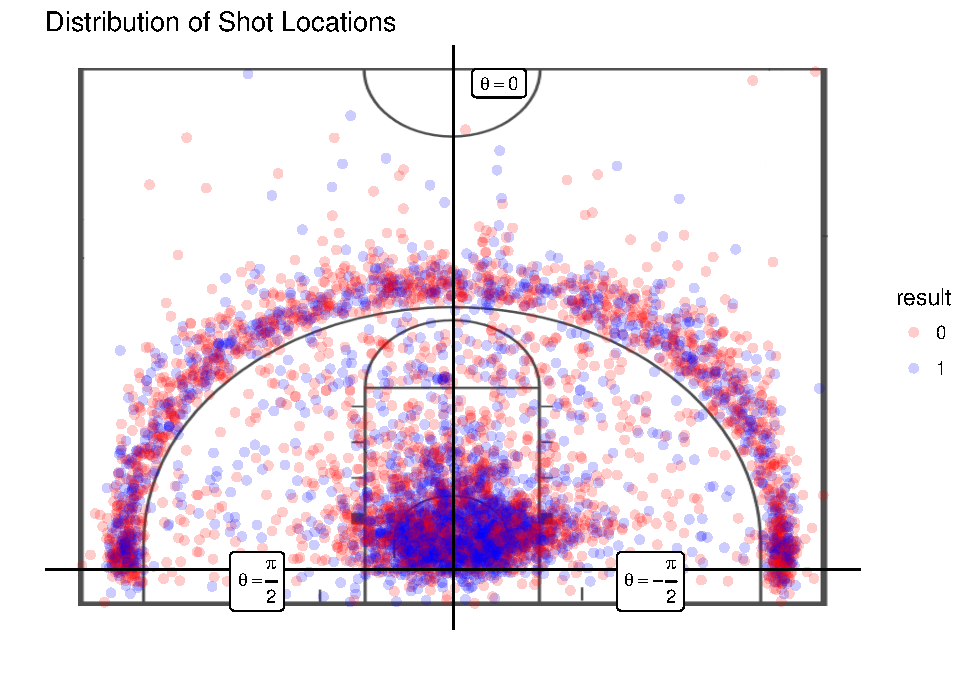
\includegraphics{thesis_files/figure-latex/shotplot-1.pdf}
\caption{\label{fig:shotplot}Locations and Results of All Shots}
\end{figure}
\section{Exploratory Data Analysis}\label{exploratory-data-analysis}

The exploratory data analysis plots in Figure \ref{fig:smoothplot}
examine how consistent the probability of a made shot is, using a loess
smooth curve on the binary outcomes. We present these smoothed plots for
four high-usage basketball players at Duke University between the 2014
and 2017 seasons. Each plot represents a single player's ordered
shooting outcomes for a single season. These plots do not account for
the amount of time in between shots, but simply shot order and outcome.
\begin{center}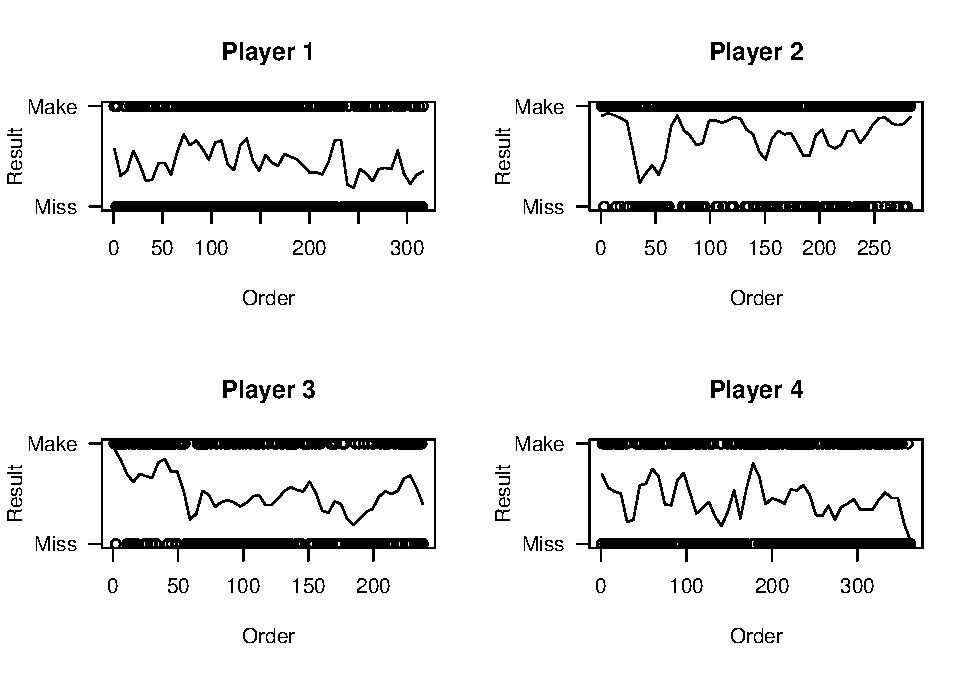
\includegraphics{thesis_files/figure-latex/smoothplot0-1} \end{center}
\begin{figure}

{\centering 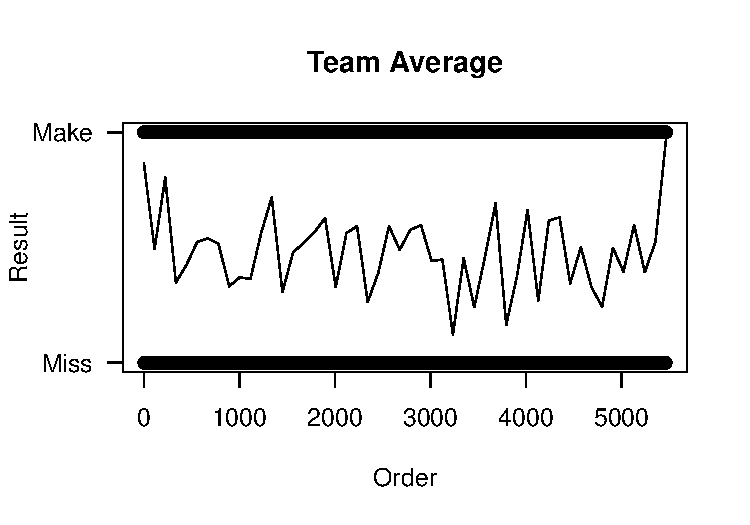
\includegraphics{thesis_files/figure-latex/smoothplot-1} 

}

\caption{Moving Average of Shot Success Rate}\label{fig:smoothplot}
\end{figure}
\pagebreak

We can see that the players vary in the consistency of their made shots,
since they all contain spikes and trends. For example, Player 3
initially has a very high success rate, which quickly falls to the
middle after about 30 shot attempts, and the Player 2 has a noticeable
upward trend in shot success beginning around shot number 150.

We investigate the shooting outcomes using Bayesian models, and present
the results in the next chapter.

\chapter{Models \& Analysis}\label{models}

\section{Description of Models}\label{description-of-models}

For our models, we consider the shot location, a home court indicator,
the shooter's identity, and his shooting outcomes in nearby games as
factors that can affect a shot's outcome. We use the Just Another Gibbs
Sampler library in R (\texttt{R2jags}) to build these models. Each one
is based on a logistic regression model that provides the posterior
distribution of the shot location parameters (distance and angle) and an
additional intercept to capture the influence of home-court advantage.
The models do not account for covariance between these predictors. We
expand upon this model by adding mixed effects and discounted likelihood
models to control for shooter identity and between-game variability,
respectively. In our Gibbs Samplers, we estimate the posterior
distributions using 10,000 simulations and a burn-in of 500. Our prior
distributions are constructed from the corresponding maximum likelihood
estimates for the first four games in the dataset, and we initialize our
Monte Carlo Markov Chains using values of 0 for all means, and 1 for all
variances. The \texttt{R2jags} code used to build these models can be
found in Appendix A.

\subsection{Generalized Linear Model}\label{generalized-linear-model}

We start with a logistic regression model for each shot attempt \(i\):

\[
\text{logit}(p_{i}) = 
\beta_{\text{int}} +
x_{\text{r,i}}\beta_{\text{r}} +
x_{\theta,\text{i}}\beta_{\theta} +
x_{\text{H,i}}\beta_{\text{H}}.
\]

In this model, the \(x\) refers to the data, and the \(\beta\)s are the
parameters from the model. The subscripts \(\textit{int}\),
\(\textit{r}\), \(\theta\), and \(\textit{H}\) respectively refer to the
intercept, the log-distance of the shot, the angle of the shot, and
whether shot was taken on Duke's home court or another gym. This fourth
\(\beta\) accounts for the possibility of ``home-court advantage'',
which can affect shot outcomes.

\subsection{Hierarchical Generalized Linear
Model}\label{hierarchical-generalized-linear-model}

Our second model is a hierarchical model, with random effects on the
\(\textit{j}\) players in the dataset. These random effects occur for
each of the four parameters of interest---the intercept, the distance
effect, the angle effect, and the home effect. Each individual player's
parameter values are sampled from a Normal distribution centered at the
population values. A benefit of this type of model is that the
parameters for players with few shot attempts are shrunk towards the
population means. The model has the form below for each player \(j\) and
shot attempt \(i\):

\[
\text{logit}(p_{\text{ji}}) = 
\beta_{\text{int, j}} +
x_{\text{r,ji}}\beta_{\text{r, j}} +
x_{\theta,\text{ji}}\beta_{\theta, \text{j}} +
x_{\text{H, ji}}\beta_{\text{H, j}},
\] \[
\beta_{\text{int, j}} \sim N(\beta_{\text{int}}, \tau^2_{\text{int}}),
\] \[
\beta_{\text{r, j}} \sim N(\beta_{\text{r}}, \tau^2_{\text{r}}),
\] \[
\beta_{\theta, j} \sim N(\beta_{\theta}, \tau^2_{\theta}),
\] \[
\beta_{\text{H, j}} \sim N(\beta_{\text{H}}, \tau^2_{\text{H}}).
\]

\subsection{Discounted Likelihood Hierarchical
Model}\label{discounted-likelihood-hierarchical-model}

In the discounted likelihood models, the likelihood function for all
model parameters at a given time is more heavily influenced by the
observations close to that specific time point than the observations far
away from it. We measure the ``distance'' between observations by the
number of games between them; a shot attempt that occurs in the next or
the preceding game will influence the likelihood function for the
parameters ``anchored'' at that game more than a shot that occurs two
games away. We chose to analyze time-dependency in the data using a
discounted likelihood model instead of a full dynamic model because a
discounted likelihood model would have fewer complications in the
context of a hierarchical model. The methodology behind our discounted
likelihood model relates closely to Bayesian dynamic modeling that uses
power discounting to reduce the effect of data that occurs further in
the past. We begin defining this model with the concept of forward
filtering. This is implied by a power-discount Bayesian time series
model (Smith, 1979) that uses a ``discounted'' Bayes Theorem in which
the posterior disitribution of the model parameters at any chosen time
\(t\) is proportional to the product of the prior, \(p(\Theta)\), and
the discount likelihood function, which has the form

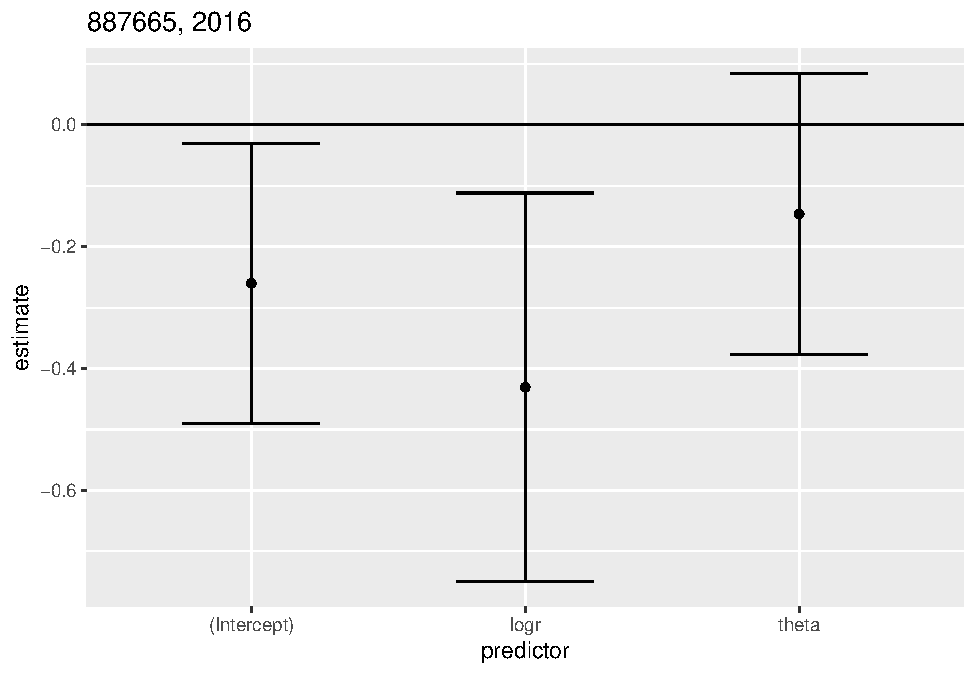
\includegraphics{thesis_files/figure-latex/unnamed-chunk-1-1.pdf}

\pagebreak

\[
p_t(X_{1:t}|\Theta) = p_t(X_{1:t-1}|\Theta)p(X_t|\Theta),
\]

where

\[
p_t(X_{1:t-1}|\Theta) \propto
p(X_{1}  |\Theta)^{\delta^{t-1}}...
p(X_{t-2}|\Theta)^{\delta^{2}}
p(X_{t-1}|\Theta)^{\delta}
\]

for some discount factor \(0 < \delta < 1\), typically closer to 1 to
allow for the discounting of past data without omitting its information
content.

This equation shows that as distance increases backward in time, the
effect on the likelihood function---and hence on the resulting posterior
for \(\Theta\) at our current time \(t\)---decreases. The corresponding
discount likelihood for \(\Theta\) at time \(t\) given both past and
future data up to a time \(T > t\) has a similar form, but with
two-sided discounting. This relates to dynamic models with time-varying
parameters, which apply backwards updating to update their posteriors.
The form of the two-sided likelihood function of \(\Theta\) at a chosen
time \(t\) is:

\[
p_t(X_{1:T}|\Theta) = 
p_t(X_{1:t-1}|\Theta)
p(X_{t}|\Theta)
p_t(X_{t+1:T}|\Theta),
\]

where the past data component \(p_t(X_{1:t-1}|\Theta)\) is the same as
above, and the future data component is:

\[
p_t(X_{t+1:T}|\Theta) \propto
p(X_{t+1}|\Theta)^{\delta}
p(X_{t+2}|\Theta)^{\delta^2}...
p(X_{T}|\Theta)^{\delta^{T-t}}.
\]

Specifically for our model, given an observed shot \(\textit{i}\) in
game \(g\), attempted by player \(\textit{j}\), we apply the above
reasoning to discount the likelihood of a made shot in the hierarchical
model. First we begin with a hierarchical logistic regression model:

\[
\text{logit}(p_{\text{gji}}) = 
\beta_{\text{int, gj}} +
x_{\text{r,gji}}\beta_{\text{r, gj}} +
x_{\theta,\text{gji}}\beta_{\theta, \text{gj}} +
x_{\text{H, gji}}\beta_{\text{H, gj}},
\] \[
\beta_{\text{int, j}} \sim N(\beta_{\text{int}}, \tau^2_{\text{int}}),
\] \[
\beta_{\text{r, j}} \sim N(\beta_{\text{r}}, \tau^2_{\text{r}}),
\] \[
\beta_{\theta, j} \sim N(\beta_{\theta}, \tau^2_{\theta}),
\] \[
\beta_{\text{H, j}} \sim N(\beta_{\text{H}}, \tau^2_{\text{H}}).
\]

Without discounting, the likelihood term controbuted from a shot's
outcome, \(\text{y}_\text{gji}\), that is attempted by player
\(\textit{j}\) in game \(\textit{g}\), is:

\[
L_\text{gj}(\Theta) =
\prod_{\text{i}=1}^{\text{n}_\text{gj}}{
  p(\text{y}_{\text{gji}} | \Theta) 
}
\propto 
\prod_{\text{i}=1}^{\text{n}_\text{gj}}{
  p_\text{gji}^{\text{y}_\text{gji}} 
  (1 - p_\text{gji})^{1-\text{y}_\text{gji}}
}.
\]

When we apply the exponential discounting to the outcomes like so:

\[
\pi_{\text{gji}} =
\left(
  p_\text{gji}^{\text{y}_\text{gji}} 
  (1 - p_\text{gji})^{1-\text{y}_\text{gji}}
\right)
^{\delta^{|g-g_0|}},
\]

our likelihood becomes:

\[
\Lambda_{\text{gj}}(\Theta) = 
\prod_{\text{i}=1}^{\text{n}_\text{gj}}
  \pi_{\text{gji}},
\]

where \({g}\) is the game index of the current shot \(\textit{i}\), and
\(g_0\) is a fixed game index, which we refer to as the ``anchor game''.

In this model, \(p\) represents the binomial probability, and \(\pi\) is
the discounted probability. Both of these quantities are probabilities
that are bounded in the interval {[}0,1{]}. Similarly, \(L\) is the
likelihood and \(\Lambda\) is the discounted likelihood. The
contribution of shot outcomes from games \(g\) that are more distant
from the anchor game \(g_0\) are more heavily discounted, and the
discounting increases for smaller values of \(\delta\). In a model with
\(\delta\) = 0, only shots taken in the same game as shot \(i\) can
contribute to the likelihood, while \(\delta\) = 1 is equivalent to a
model with no discounting. If models with larger values of \(\delta\)
best fit the data, this suggests that shooting success is consistent
throughout a career. If smaller values of \(\delta\) are more likely in
the data, however, then we can assume there is a substantial amount of
time variation, or ``streakiness'', in the data on the game level.
Figure \ref{fig:discplot} illustrates how the exponential weight on the
likelihood depends on the selected value of \(\delta\) and the distance
from the anchor game (\(g - g_0\)).


\includegraphics{thesis_files/figure-latex/unnamed-chunk-2-1.pdf}

\pagebreak
\begin{figure}[htbp]
\centering
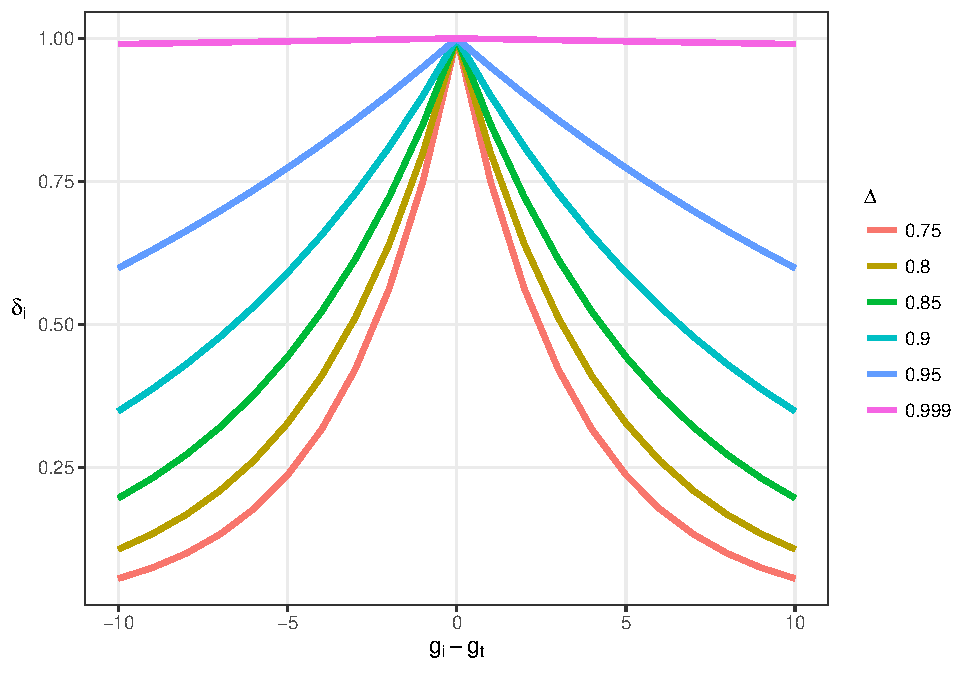
\includegraphics{thesis_files/figure-latex/discplot-1.pdf}
\caption{\label{fig:discplot}Illustration of Discounted Weighting}
\end{figure}
This model specification is specific to the chosen anchor game \(g_0\),
so that the resulting posterior distribution for all model parameters is
indexed by \(g_0\) and represents inferences ``local'' to that game.
Repeating the analysis across all games as anchors results in a sequence
of posteriors, where their differences reflect time variation. As a
result, we refit the model using MCMC for each combination of game index
and \(\delta\), which involves substantial computation.


\includegraphics{thesis_files/figure-latex/unnamed-chunk-3-1.pdf}

\pagebreak

To build these discounted likelihood models in the \texttt{R2jags}
library, we apply the ``ones trick''. This technique allows us to use a
sampling distribution that does not exist in the library by modifying a
common distribution---in this case, the Binomial. The probability \(p\)
is estimated in the same way as the Bayesian hierarchical model. We
discount this probability to estimate \(\pi\), and then we specify that
it comes from Binomial data that consists only of ones; this is
equivalent to sampling from a distribution with discounted outcomes. In
the code excerpt below, \texttt{result} and \texttt{prob} are the
binomial outcomes and probabilities, while \texttt{y} represents the
``trick'' outcomes (a vector of 1s), and \texttt{pi} is the discounted
probability.


\includegraphics{thesis_files/figure-latex/unnamed-chunk-4-1.pdf}
\begin{Shaded}
\begin{Highlighting}[]
    \NormalTok{for(i in }\DecValTok{1}\NormalTok{:N)\{}
      
      \CommentTok{# delta = discount rate for game g relative to anchor game g0}
      \NormalTok{wt[i] <-}\StringTok{ }\NormalTok{delta^}\KeywordTok{abs}\NormalTok{(games[i]-g0)  }
      
      \CommentTok{# player-level random effects}
      \KeywordTok{logit}\NormalTok{(prob[i]) <-}\StringTok{ }\NormalTok{beta_int[player[i]]*int[i] +}\StringTok{ }
\StringTok{                        }\NormalTok{beta_home[player[i]]*home[i] +}\StringTok{ }
\StringTok{                        }\NormalTok{beta_r[player[i]]*logr[i] +}\StringTok{ }
\StringTok{                        }\NormalTok{beta_theta[player[i]]*theta[i] }

      \CommentTok{# likelihood function}
      \NormalTok{p1[i] <-}\StringTok{ }\NormalTok{prob[i]^result[i]}
      \NormalTok{p2[i] <-}\StringTok{ }\NormalTok{(}\DecValTok{1}\NormalTok{-prob[i])^(}\DecValTok{1}\NormalTok{-result[i])}
      
      \CommentTok{# discounted likelihood function}
      \NormalTok{pi[i] <-}\StringTok{ }\NormalTok{(p1[i] *}\StringTok{ }\NormalTok{p2[i])^wt[i]  }
      
      \CommentTok{# defines correct discounted likelihood function}
      \NormalTok{y[i] ~}\StringTok{ }\KeywordTok{dbern}\NormalTok{(pi[i]) }
      
    \NormalTok{\}}
    
    \CommentTok{# Priors}
    \NormalTok{for(j in }\DecValTok{1}\NormalTok{:M)\{}
      \NormalTok{beta_int[j] ~}\StringTok{ }\KeywordTok{dnorm}\NormalTok{(beta_int0,tau_int)}
      \NormalTok{beta_home[j] ~}\StringTok{ }\KeywordTok{dnorm}\NormalTok{(beta_home0, tau_int)}
      \NormalTok{beta_r[j] ~}\StringTok{ }\KeywordTok{dnorm}\NormalTok{(beta_r0,tau_r)}
      \NormalTok{beta_theta[j] ~}\StringTok{ }\KeywordTok{dnorm}\NormalTok{(beta_theta0,tau_theta)}
    \NormalTok{\}}
\end{Highlighting}
\end{Shaded}
See Appendix A.3 for the full \texttt{R} code.

\section{Analysis}\label{analysis}

\subsection{Generalized Linear Model}\label{generalized-linear-model-1}

In our generalized linear model, we only look at shot location and the
home court indicator as predictors of shot outcome. This is a logistic
regression model where the intercepts correspond to the log-odds of
making a shot when the angle is zero (the middle of the court) and the
log-distance is zero (one foot away from the rim). To illustrate these
effects for individual players, we simply subset the dataset to include
only shots attempted by that player before running the Gibbs Sampler. In
Figure \ref{fig:glmplot}, The 95\% credible intervals of the posterior
parameters are reported for the same four players that were introduced
in Figure \ref{fig:smoothplot}.


\includegraphics{thesis_files/figure-latex/unnamed-chunk-6-1.pdf}
\begin{center}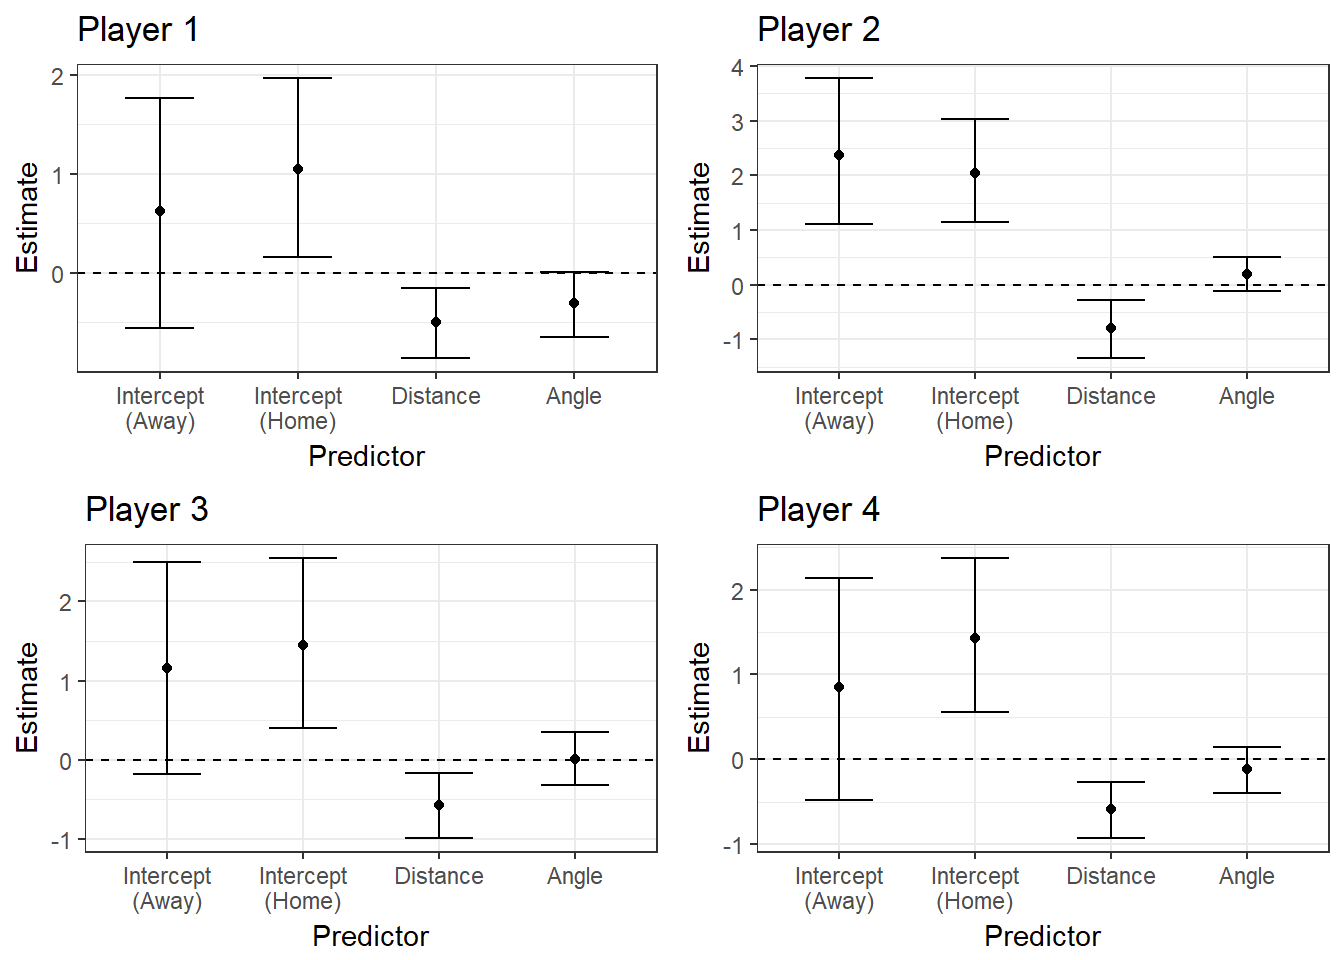
\includegraphics{thesis_files/figure-latex/glmplot0-1} \end{center}
\begin{figure}

{\centering 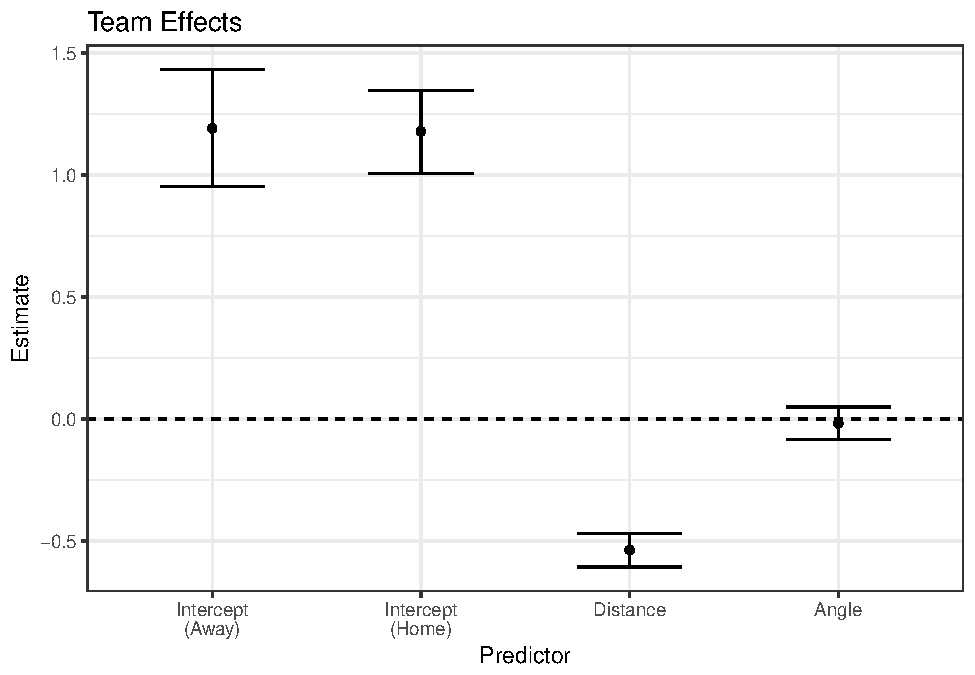
\includegraphics{thesis_files/figure-latex/glmplot-1} 

}

\caption{GLM Posterior Distributions for Four Players}\label{fig:glmplot}
\end{figure}
From these plots, we see that the team-wide 95\% credible interval of
the angle effect is centered at zero, and it is therefore probably not
predictive of a made shot. The average distance effect shows us that the
log-odds of a made shot decrease by \(\beta_r =\) 0.5372 as the
log-distance increases by one unit and the other predictors remain
constant. This effect is translated to the probability scale using the
expression

\[
\frac{\text{e}^{\beta_r}}{1 + \text{e}^{\beta_r}},
\]

which equals 0.3689.

We also see that the 95\% credible interval on the effect of distance is
completely negative, which follows the intuitive idea that the
probability of a made shot significantly decreases as distance from the
basket increases. The intercepts show us that there is not a substantial
difference in baseline shooting performance between home games and away
games. The interval for away games is wider because there are fewer of
them in the dataset.

\subsection{Hierarchical Generalized Linear
Model}\label{hierarchical-generalized-linear-model-1}

To make the hierarchical model, we add random effects that allow the
parameters to vary for each player in the dataset. For every linear
covariate in the model, we model player-specific effects as sampled from
a Normal distribution roughly centered at the covariate's population
mean. We present the results in Figure \ref{fig:hierplot} by comparing
the effects of the four high-usage players of interest to the population
density of each covariate.

\pagebreak
\begin{figure}[htbp]
\centering
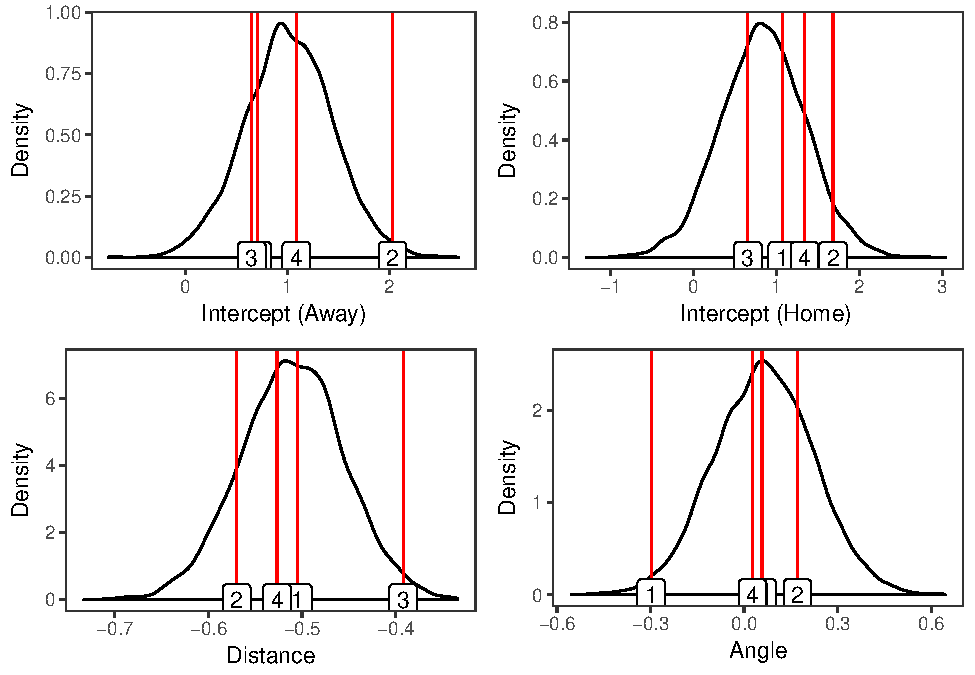
\includegraphics{thesis_files/figure-latex/hierplot-1.pdf}
\caption{\label{fig:hierplot}Population Distribution with Four Player
Effects}
\end{figure}
The plots in Figure \ref{fig:hierplot} show us that Player 2 excels at
scoring under baseline conditions (close to the basket), but he has a
steeper-than-average drop in his odds of scoring as his distance from
the basket increases. We can also see that Player 1 strongly increases
his odds of scoring when his angle is negative, which corresponds to the
left side of the basket, while the other three players' effects are all
close to zero.

In Figure \ref{fig:contplot}, we present contour plots showing the
players' expected field goal percentages at all locations on the half of
the court where they are shooting. We compute these from the fitted
probabilities of shot success from the hierarchical model. This plot
confirms that Player 1 is more effective on the left side of the basket
than the others. Other takeaways that were not noticeable in Figure
\ref{fig:hierplot} are that Player 2 has the darkest overall contour
plot, which suggests that he has the highest overall probability of
scoring, and that Player 4 has lightest plot, suggesting he is the least
reliable scorer among these four players.

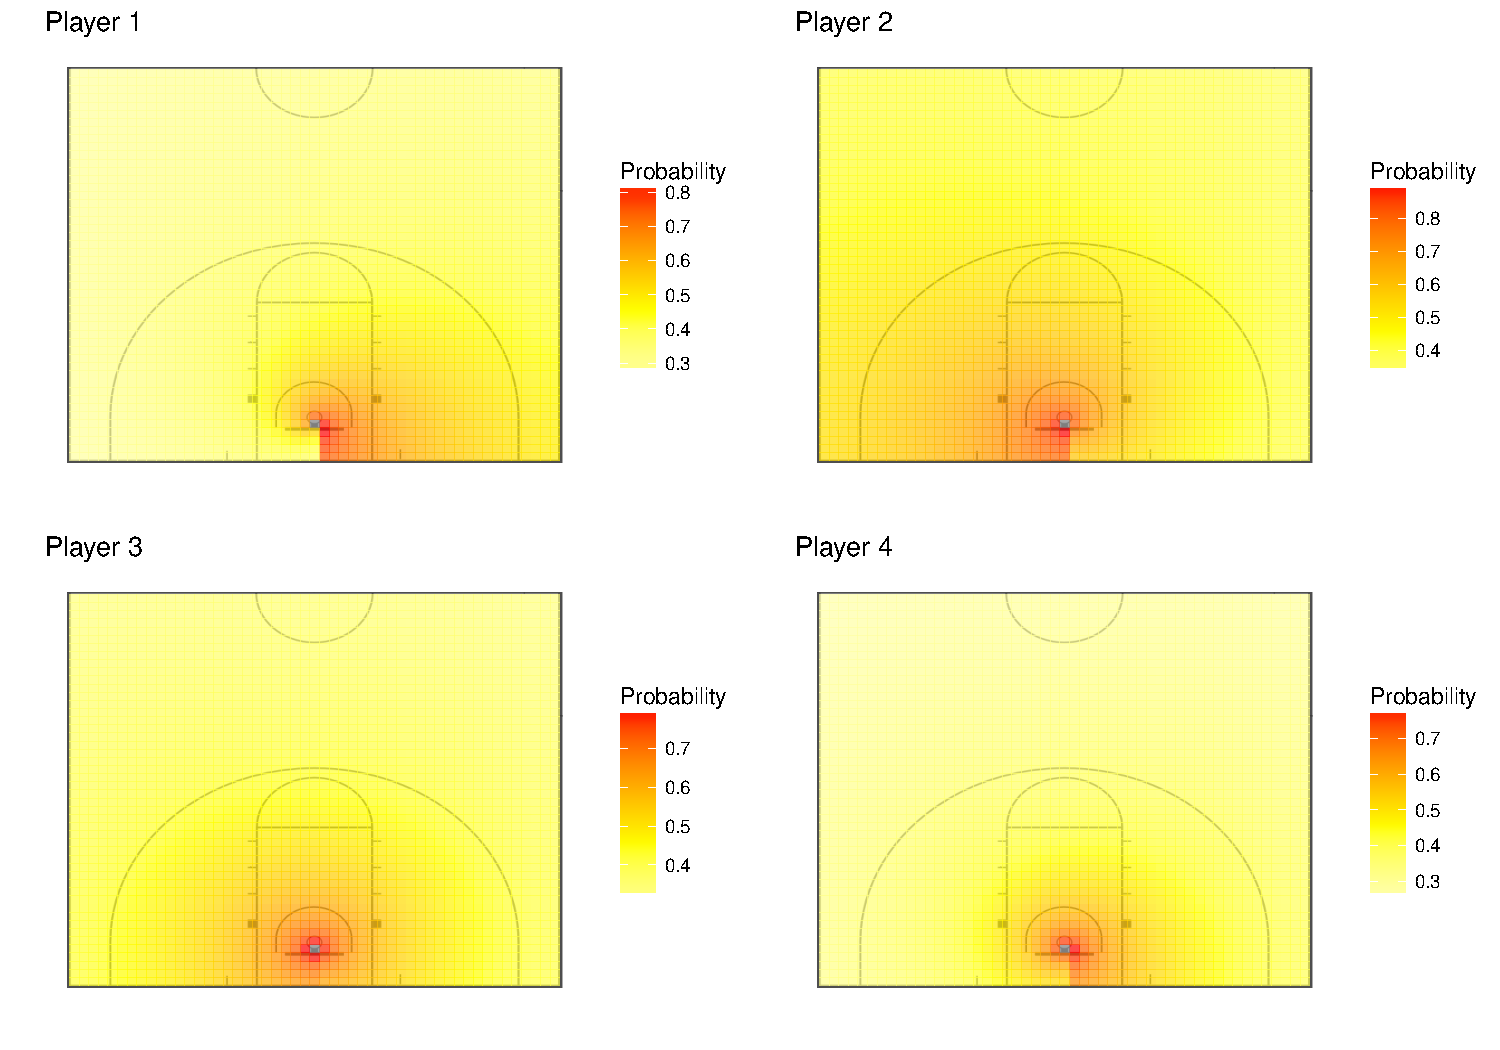
\includegraphics{thesis_files/figure-latex/contplot0-1.pdf}
\begin{figure}

\hfill{}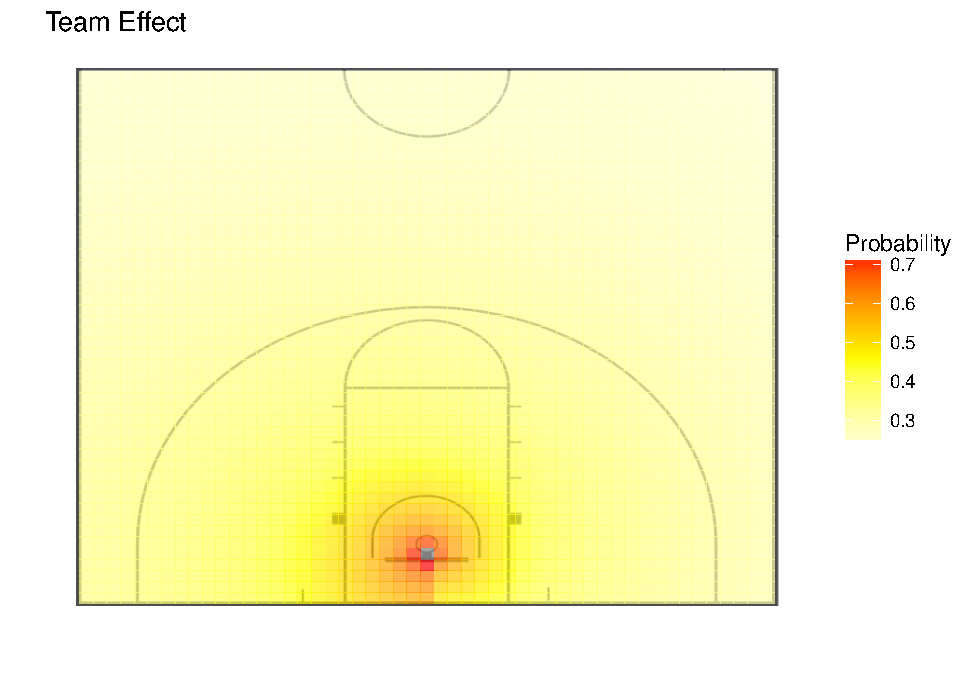
\includegraphics[width=0.9\linewidth]{thesis_files/figure-latex/contplot-1} 

\caption{Contour Plots for Four Players and Population of Players}\label{fig:contplot}
\end{figure}
\subsection{Discounted Likelihood Hierarchical
Model}\label{discounted-likelihood-hierarchical-model-1}

The values of \(\delta\) that we use to fit the discounted likelihood
models are 0.750, 0.800, 0.850, 0.900, 0.950, and 0.999. For each of
these values, we refit the model to generate a full MCMC sample from the
posterior, using every game as the anchor game \(g_0\). We calculate
predictions and fitted values for a particular shot in game \(g\) using
the posterior median of the MCMC chain where \(g\) is the anchor game
\(g_0\). The plots in Figure \ref{fig:discplot750} and
\ref{fig:discplot999} show how the posterior parameter distributions
(95\% credible intervals) change over the course of one season on the
team level and for two players (the other two players are not shown here
because they did not play during this season). Figure
\ref{fig:discplot750} illustrates the results for our smallest value of
\(\delta\), 0.750, and \ref{fig:discplot999} shows them for our largest
value of \(\delta\), 0.999.
\begin{figure}

{\centering 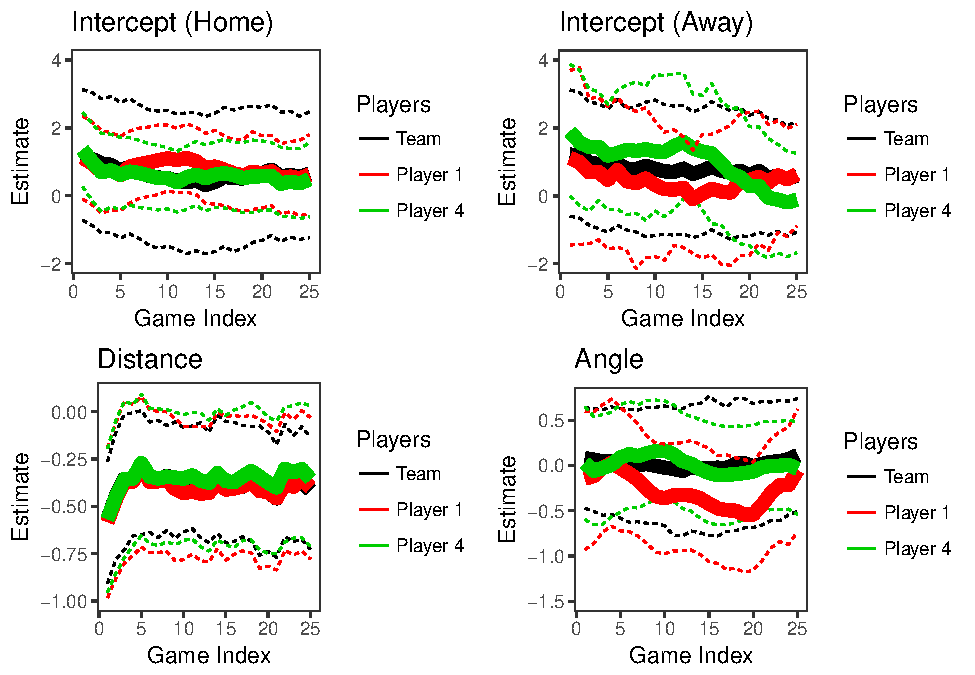
\includegraphics{thesis_files/figure-latex/discplot750-1} 

}

\caption{Parameters for Two Players and Population over Time, $\delta$ = 0.750}\label{fig:discplot750}
\end{figure}
\begin{figure}

{\centering 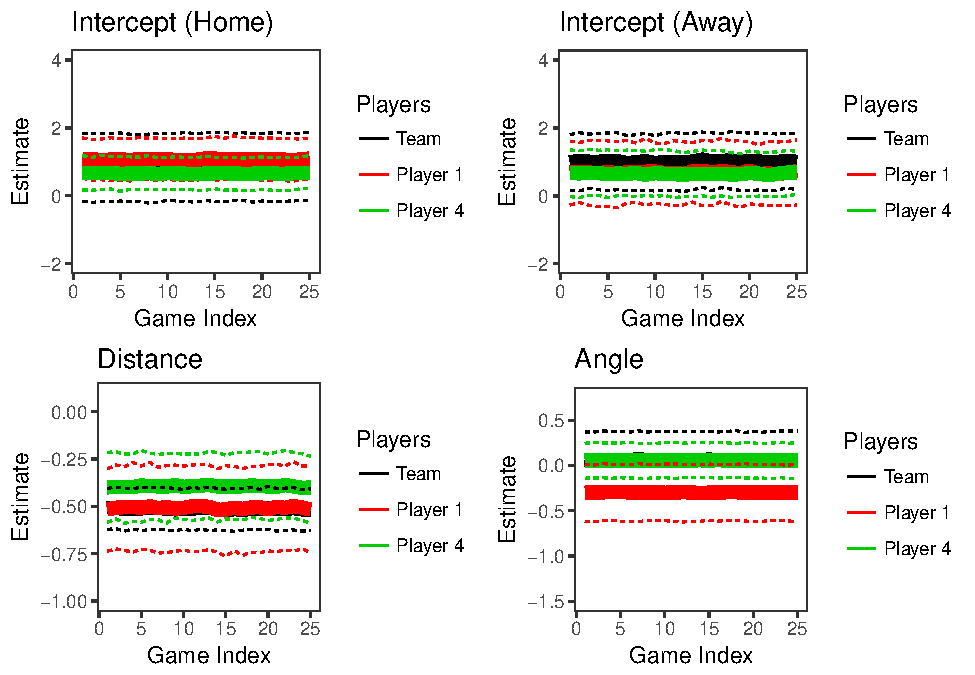
\includegraphics{thesis_files/figure-latex/discplot999-1} 

}

\caption{Parameters for Two Players and Population over Time, $\delta$ = 0.999}\label{fig:discplot999}
\end{figure}
These plots illustrate how smaller values of \(\delta\) allow for more
variation in the posteriors over time. Another observation from this
plot is that the credible intervals are wider when \(\delta\) is
smaller. Between the two plots of the home game intercepts, we can see
that the 95\% credible in the first game when \(\delta\) = 0.750 ranges
from about -1 to 3, while the corresponding interval in the plot where
\(\delta\) = 0.999 ranges from about 0 to 2. The uncertainty in the
posteriors increases as the discounting parameter \(\delta\) decreases
because a smaller \(\delta\) corresponds to fewer observations
contributing to the likelihood.

\chapter{Discussion}\label{disc}

\section{Evaluation of Models}\label{evaluation-of-models}

To evaluate these models, we use 5-fold cross-validation. In each
train-test split, we evaluate the models' out-of-sample classification
rates (using a cutoff probability of 0.5), Brier scores (mean squared
error), and log-likelihoods. The predictions and fitted values are
obtained using MCMC averages; to calculate the probability for an
individual shot, we calculate a response for each of the 9,500 posterior
simulations, then take the average of those responses. This process used
up to 20 simultaneous RStudio Pro servers provided by the Duke
University Statistical Science Department. The results are plotted below
in Figure \ref{fig:evalplot}:


\includegraphics{thesis_files/figure-latex/unnamed-chunk-7-1.pdf}

\pagebreak
\begin{figure}

{\centering 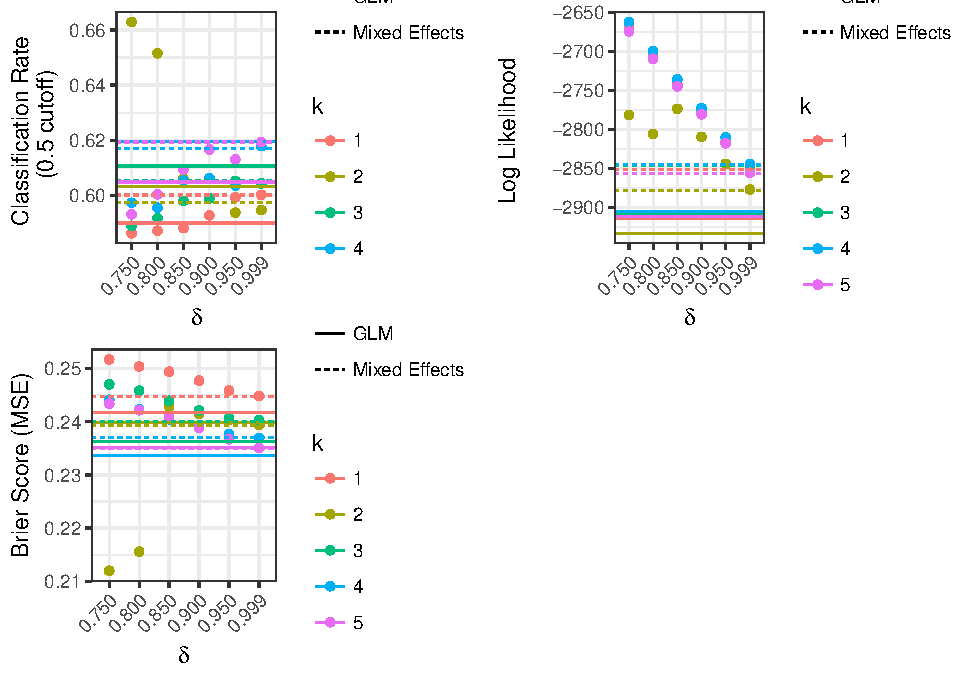
\includegraphics{thesis_files/figure-latex/evalplot-1} 

}

\caption{Model Evaluation}\label{fig:evalplot}
\end{figure}
From Figure \ref{fig:evalplot}, we can observe that all of the models
have different strengths. The discounted likelihood model with the
smallest value of \(\delta\) consistently has the highest likelihood.
However, it does not test as well as the other models in areas of
out-of-sample classification rate and Brier score. This suggests that
models with smaller values of \(\delta\), where the likelihood of an
observed shot is more heavily influenced by shots closer to it, may
overfit the model to the training data. The generalized linear models
perform best in Brier score, but worst in log-likelihood. The
hierarchical models are about the same as the GLMs, but they have a
better log-likelihood performance. A model that balances the trade-off
between predictive accuracy and likelihood is a discounted likelihood
model with \(\delta\) = 0.850.

In addition, we can see that the overall variation in model performance
is small. For example, most of the out-of-sample classification rates
fall between 0.58 and 0.62. This is within the 95\% confidence interval
for a random binomial proportion of 0.6 using a sample size of 40
(because there are 8 different models and 5 train-test splits for each
model), which is (0.5225, 0.6775). Therefore, the evidence that the
models without discounting predict better than the ones with discounting
is not particularly strong.

For the discounted likelihood model with \(\delta\) = 0.850, we build
calibration plots to assess how well the estimated probabilities fit the
actual proportions. To make these plots, we divide the predicted
probabilities into 20 equally-sized bins, then plot these bins on the
x-axis with the proportions of the actual outcomes within the bins on
the y-axis. The horizontal bars represent the bin width, and the
vertical bars represent a 95\% confidence interval of the proportions.
The red line of slope 1 represents equality between the bin medians and
the empirical probabilities within the bins. In Figure
\ref{fig:caliplot}, we present these plots for a full training set and a
testing set.
\begin{figure}[htbp]
\centering
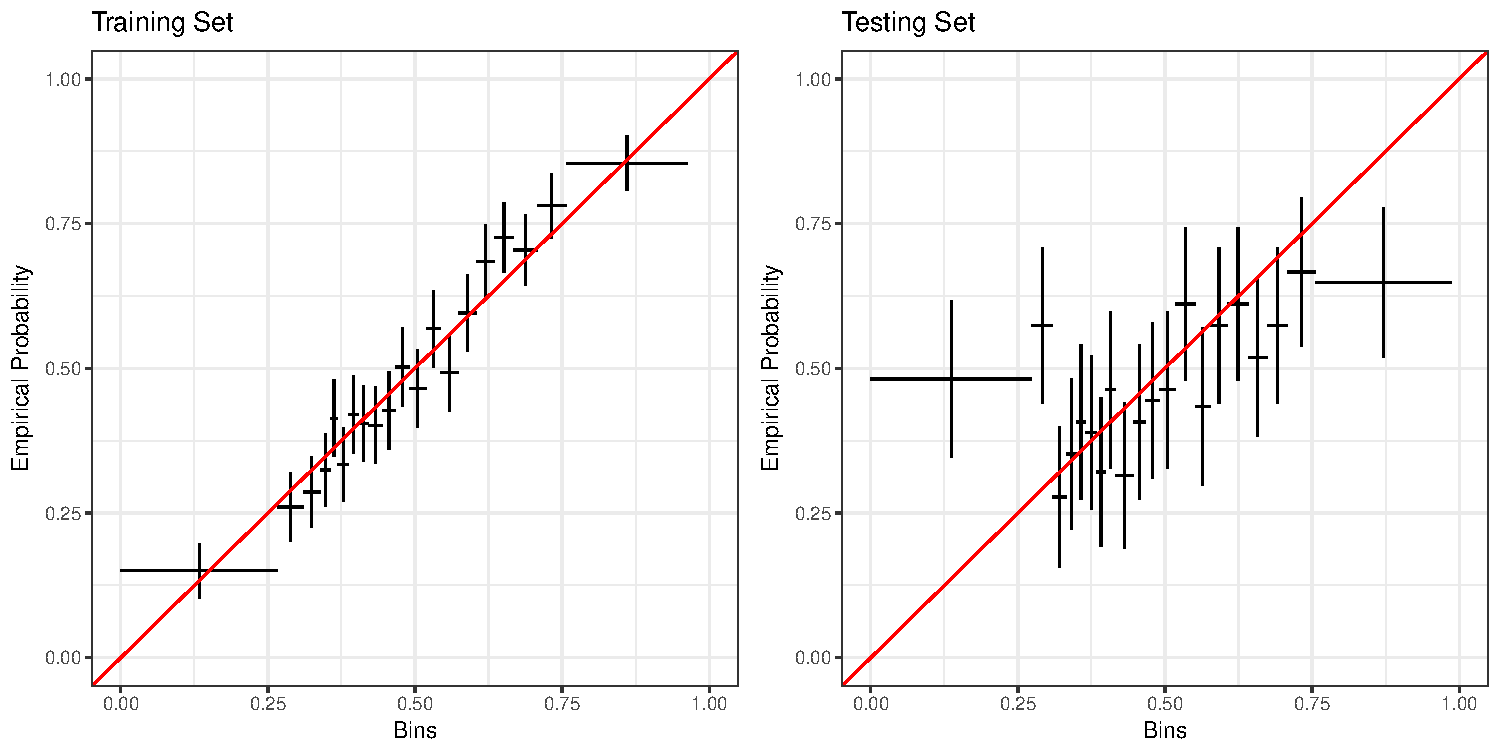
\includegraphics{thesis_files/figure-latex/caliplot-1.pdf}
\caption{\label{fig:caliplot}Calibration Plots for Discounted Likelihood
Model, \(\delta\) = 0.850}
\end{figure}
\pagebreak

We can see that the confidence intervals on the training set all cross
the line of slope 1, which shows that the model output reliably fits the
probabilities. In the testing set, however, the predictions only cross
this line between about 0.3 and 0.75. In addition, the widths of the
bins on the edges show that the model is not likely to predict values
close to 0 or 1.

\section{\texorpdfstring{Results from Model with \(\delta\) =
0.850}{Results from Model with \textbackslash{}delta = 0.850}}\label{results-from-model-with-delta-0.850}

To illustrate results from the discounted likelihood model with
\(\delta\) = 0.850, we replicate the plots in Figures
\ref{fig:discplot750} and \ref{fig:discplot999}. The results are shown
in Figure \ref{fig:discplot850}.
\begin{figure}

\hfill{}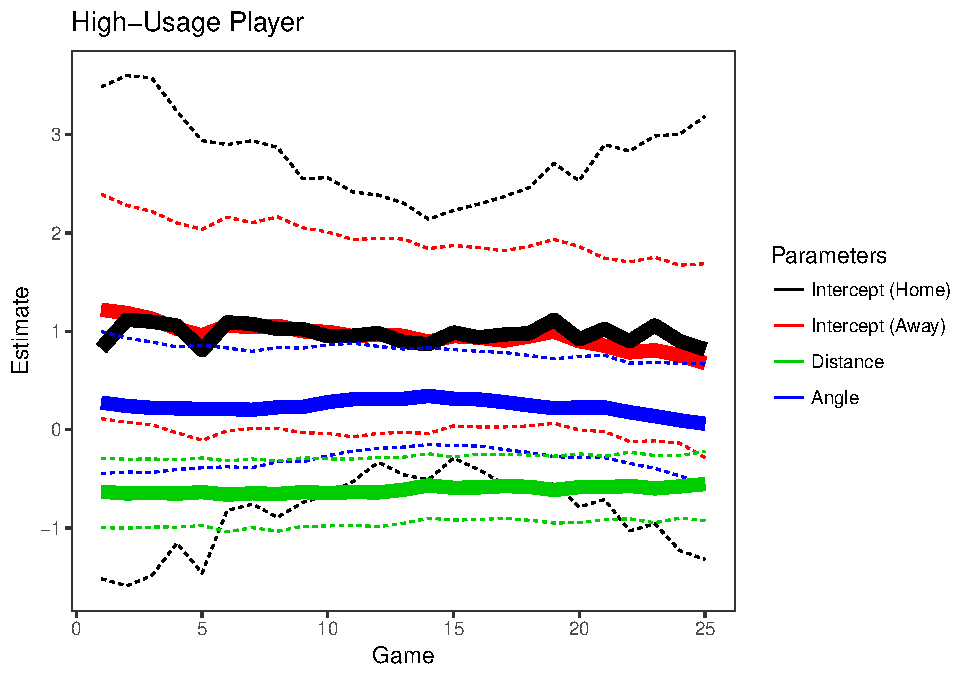
\includegraphics[width=0.9\linewidth]{thesis_files/figure-latex/discplot850-1} 

\caption{Parameters for Two Players and Population over Time, $\delta$ = 0.850}\label{fig:discplot850}
\end{figure}
Figure \ref{fig:discplot850} has smoother changes over time than in
Figure \ref{fig:discplot750}, where \(\delta\) = 0.750, which could
indicate that there is less overfitting. One surprising result from this
model is how the distance parameters slightly increase over time, and
the intercepts slightly decrease. This could be a result of team shot
selection evolving throughout the season, or just a coincidental signal.

\section{Conclusion}\label{conclusion}

The evaluations of the models show that there is some weak evidence for
time-dependency in shooting success rate in this dataset of
player-tracking data from the Duke Men's Basketball team. Allowing
predictors of shot success to shift based on recent success does not
significantly improve the predictive accuracy of a model. However, we do
see a systematic improvement in likelihood for smaller discount factors
(i.e., more emphasis on recent shots, and therefore support of
``streakiness''). Weaknesses of the discounting model include a smaller
sample size and poorer out-of-sample prediction. Takeaways that we
observed in other models include the fact that the angle of the shot
only matters for certain players, and it is not a significant predictor
of shot success between all players. Also, the effects of home-court
advantage are not strong in this dataset, possibly due to the fact that
most of the games away from home are missing.

To account for possible unexplained variation between seasons, and for
variation introduced from having such a small population of road games,
I repeated this analysis on a subset of the data that only consisted of
shots from available games in one season (25 games), and shots from all
home games (82 games). The results were similar, except for increased
uncertainty due to smaller sample sizes. The model evaluation plots show
similar patterns to the ones in Figure \ref{fig:evalplot}, and they are
presented in Appendix B.

\section{Future Goals}\label{future-goals}

Future goals for this research are to build a better-fitting model to
predict basketball shots using more advanced factors that can be
approximated from the dataset. Possibilities for this include
reparametrizing the location of a shot using categories (e.g., corner
three-point shots, heaves from half-court) using the distance of the
nearest defender as a proxy for defense quality, or using the amount of
time a player has played without a substitution or timeout to
approximate fatigue. In addition, we make the unrealistic assumption
that every player exhibits the same amount of shooting streakiness with
our discounted likelihood models. We could improve upon this assumption
in the discounted likelihood models by adding a random effect on
\(\delta\), to allow it to vary by player.

\appendix

\chapter{Code for Models}\label{code-for-models}

\section{Generalized Linear Model}\label{generalized-linear-model-2}
\begin{Shaded}
\begin{Highlighting}[]
\NormalTok{Xtrainsub <-}\StringTok{ }
\StringTok{  }\NormalTok{Xtrain %>%}\StringTok{ }
\StringTok{  }\KeywordTok{filter}\NormalTok{(}\KeywordTok{as.integer}\NormalTok{(}\KeywordTok{as.factor}\NormalTok{(gameid)) <}\StringTok{ }\DecValTok{5}\NormalTok{)}

\NormalTok{priormod <-}\StringTok{ }\KeywordTok{glm}\NormalTok{(}\DataTypeTok{formula =} \NormalTok{result ~}\StringTok{ }\KeywordTok{log}\NormalTok{(r) +}\StringTok{ }\NormalTok{theta, }
                \DataTypeTok{data =} \NormalTok{Xtrainsub, }
                \DataTypeTok{family =} \StringTok{"binomial"}\NormalTok{)}

\NormalTok{mu0r <-}\StringTok{ }\KeywordTok{summary}\NormalTok{(priormod)[[}\StringTok{"coefficients"}\NormalTok{]][}\StringTok{"log(r)"}\NormalTok{,}\StringTok{"Estimate"}\NormalTok{]}
\NormalTok{mu0theta <-}\StringTok{ }\KeywordTok{summary}\NormalTok{(priormod)[[}\StringTok{"coefficients"}\NormalTok{]][}\StringTok{"theta"}\NormalTok{,}\StringTok{"Estimate"}\NormalTok{]}

\NormalTok{fit_glm <-}\StringTok{ }\NormalTok{function(dat, }\DataTypeTok{S =} \DecValTok{10000}\NormalTok{, }\DataTypeTok{B =} \DecValTok{500}\NormalTok{)\{}

  \NormalTok{model.glm <-}\StringTok{ }\NormalTok{function()\{}
  
    \CommentTok{# Liklihood function (for N observations)}
    \NormalTok{for(i in }\DecValTok{1}\NormalTok{:N)\{}
      
      \KeywordTok{logit}\NormalTok{(prob[i]) <-}\StringTok{ }\NormalTok{beta_int*int[i] +}\StringTok{ }
\StringTok{        }\NormalTok{beta_home*home[i] +}
\StringTok{        }\NormalTok{beta_r*logr[i] +}\StringTok{ }
\StringTok{        }\NormalTok{beta_theta*theta[i]}
      
      \NormalTok{result[i] ~}\StringTok{ }\KeywordTok{dbern}\NormalTok{(prob[i])}
    \NormalTok{\}}

    \CommentTok{# Priors}
    \CommentTok{# we expect less variation in the distance parameter, }
    \CommentTok{# because shot success rate should get worse }
    \CommentTok{# as distance increases under baseline circumstances.}
    \NormalTok{beta_int   ~}\StringTok{ }\KeywordTok{dnorm}\NormalTok{(}\DecValTok{0}\NormalTok{, }\FloatTok{0.1}\NormalTok{)}
    \NormalTok{beta_home  ~}\StringTok{ }\KeywordTok{dnorm}\NormalTok{(}\DecValTok{0}\NormalTok{, }\FloatTok{0.1}\NormalTok{)}
    \NormalTok{beta_r     ~}\StringTok{ }\KeywordTok{dnorm}\NormalTok{(mu0r, }\FloatTok{0.01}\NormalTok{) }
    \NormalTok{beta_theta ~}\StringTok{ }\KeywordTok{dnorm}\NormalTok{(mu0theta, }\FloatTok{0.1}\NormalTok{)}
  \NormalTok{\}}

  \NormalTok{datlist.glm <-}\StringTok{  }
\StringTok{    }\KeywordTok{list}\NormalTok{(}
      \DataTypeTok{int =} \KeywordTok{rep}\NormalTok{(}\DecValTok{1}\NormalTok{, }\KeywordTok{nrow}\NormalTok{(dat)),}
      \DataTypeTok{logr =} \KeywordTok{log}\NormalTok{(dat$r), }
      \DataTypeTok{theta =} \NormalTok{dat$theta, }
      \DataTypeTok{result =} \NormalTok{dat$result,}
      \DataTypeTok{home =} \NormalTok{dat$home,}
      \DataTypeTok{N =} \KeywordTok{nrow}\NormalTok{(dat), }
      \DataTypeTok{mu0r =} \NormalTok{mu0r,}
      \DataTypeTok{mu0theta =} \NormalTok{mu0theta}
    \NormalTok{)}
  
  \NormalTok{params.glm <-}\StringTok{ }\KeywordTok{c}\NormalTok{(}\StringTok{"beta_int"}\NormalTok{,}
                  \StringTok{"beta_home"}\NormalTok{,}
                  \StringTok{"beta_r"}\NormalTok{,}
                  \StringTok{"beta_theta"}\NormalTok{)}

  \NormalTok{initslist <-}\StringTok{ }\KeywordTok{list}\NormalTok{(}\KeywordTok{list}\NormalTok{(}\StringTok{"beta_int"}\NormalTok{=}\DecValTok{0}\NormalTok{, }
                         \StringTok{"beta_r"}\NormalTok{=}\DecValTok{0}\NormalTok{, }
                         \StringTok{"beta_theta"}\NormalTok{=}\DecValTok{0}\NormalTok{, }
                         \StringTok{"beta_home"}\NormalTok{=}\DecValTok{0}\NormalTok{))}
                    
  \NormalTok{sim <-}\StringTok{ }
\StringTok{    }\KeywordTok{jags}\NormalTok{(}\DataTypeTok{data =} \NormalTok{datlist.glm, }
         \DataTypeTok{n.chains =} \DecValTok{1}\NormalTok{, }\DataTypeTok{n.iter =} \NormalTok{S, }\DataTypeTok{n.burnin =} \NormalTok{B, }\DataTypeTok{n.thin =} \DecValTok{1}\NormalTok{,}
         \DataTypeTok{inits=}\NormalTok{initslist,}
         \DataTypeTok{parameters.to.save =} \NormalTok{params.glm,}
         \DataTypeTok{model.file=}\NormalTok{model.glm}
    \NormalTok{)}
  
  \NormalTok{sim.mcmc <-}\StringTok{ }\KeywordTok{as.data.frame}\NormalTok{(}\KeywordTok{as.mcmc}\NormalTok{(sim)[[}\DecValTok{1}\NormalTok{]])}
  
  \CommentTok{# Changing from a baseline mean + a shift amount}
  \CommentTok{# to two different means based on the type of game.}
  \NormalTok{sim.mcmc <-}\StringTok{ }
\StringTok{    }\NormalTok{sim.mcmc %>%}\StringTok{ }
\StringTok{    }\KeywordTok{mutate}\NormalTok{(}\DataTypeTok{beta_intA =} \NormalTok{beta_int,}
           \DataTypeTok{beta_intH =} \NormalTok{beta_int +}\StringTok{ }\NormalTok{beta_home) %>%}
\StringTok{    }\KeywordTok{select}\NormalTok{(beta_intA, beta_intH, beta_r, beta_theta)}
  
  \KeywordTok{return}\NormalTok{(sim.mcmc)}
\NormalTok{\}}
\end{Highlighting}
\end{Shaded}
\section{Hierarchical Generalized Linear
Model}\label{hierarchical-generalized-linear-model-2}
\begin{Shaded}
\begin{Highlighting}[]
\NormalTok{Xtrainsub <-}\StringTok{ }
\StringTok{  }\NormalTok{Xtrain %>%}\StringTok{ }
\StringTok{  }\KeywordTok{filter}\NormalTok{(}\KeywordTok{as.integer}\NormalTok{(}\KeywordTok{as.factor}\NormalTok{(gameid)) <}\StringTok{ }\DecValTok{5}\NormalTok{)}

\NormalTok{priormod <-}\StringTok{ }\KeywordTok{glm}\NormalTok{(}\DataTypeTok{formula =} \NormalTok{result ~}\StringTok{ }\KeywordTok{log}\NormalTok{(r) +}\StringTok{ }\NormalTok{theta, }
                \DataTypeTok{data =} \NormalTok{Xtrainsub, }
                \DataTypeTok{family =} \StringTok{"binomial"}\NormalTok{)}

\NormalTok{mu0r <-}\StringTok{ }\KeywordTok{summary}\NormalTok{(priormod)[[}\StringTok{"coefficients"}\NormalTok{]][}\StringTok{"log(r)"}\NormalTok{,}\StringTok{"Estimate"}\NormalTok{]}
\NormalTok{mu0theta <-}\StringTok{ }\KeywordTok{summary}\NormalTok{(priormod)[[}\StringTok{"coefficients"}\NormalTok{]][}\StringTok{"theta"}\NormalTok{,}\StringTok{"Estimate"}\NormalTok{]}

\NormalTok{fit_players <-}\StringTok{ }\NormalTok{function(}\DataTypeTok{dat =} \OtherTok{NA}\NormalTok{, }\DataTypeTok{S =} \DecValTok{10000}\NormalTok{, }\DataTypeTok{B =} \DecValTok{500}\NormalTok{)\{}
  
  \NormalTok{model.player <-}\StringTok{ }\NormalTok{function()\{}
    
    \CommentTok{# Likelihood function for N observations}
    \NormalTok{for(i in }\DecValTok{1}\NormalTok{:N)\{}
      
      \CommentTok{# the parameters now vary by player id.}
      \KeywordTok{logit}\NormalTok{(prob[i]) <-}\StringTok{ }\NormalTok{beta_int[player[i]]*int[i] +}\StringTok{ }
\StringTok{        }\NormalTok{beta_home[player[i]]*home[i] +}\StringTok{ }
\StringTok{        }\NormalTok{beta_r[player[i]]*logr[i] +}\StringTok{ }
\StringTok{        }\NormalTok{beta_theta[player[i]]*theta[i]}
      
      \NormalTok{result[i] ~}\StringTok{ }\KeywordTok{dbern}\NormalTok{(prob[i])}
    \NormalTok{\}}
    
    \CommentTok{# Priors}
    \NormalTok{for(j in }\DecValTok{1}\NormalTok{:M)\{}
        \NormalTok{beta_int[j] ~}\StringTok{ }\KeywordTok{dnorm}\NormalTok{(beta_int0,tau_int)}
        \NormalTok{beta_home[j]  ~}\StringTok{ }\KeywordTok{dnorm}\NormalTok{(beta_home0, tau_int)}
        \NormalTok{beta_r[j] ~}\StringTok{ }\KeywordTok{dnorm}\NormalTok{(beta_r0,tau_r)}
        \NormalTok{beta_theta[j] ~}\StringTok{ }\KeywordTok{dnorm}\NormalTok{(beta_theta0,tau_theta)}
    \NormalTok{\}}
    
    \CommentTok{# Hyperpriors}
    \NormalTok{beta_int0   ~}\StringTok{ }\KeywordTok{dnorm}\NormalTok{(}\DecValTok{0}\NormalTok{, }\FloatTok{0.1}\NormalTok{)}
    \NormalTok{beta_home0  ~}\StringTok{ }\KeywordTok{dnorm}\NormalTok{(}\DecValTok{0}\NormalTok{, }\FloatTok{0.1}\NormalTok{)}
    \NormalTok{beta_r0     ~}\StringTok{ }\KeywordTok{dnorm}\NormalTok{(mu0r, }\FloatTok{0.01}\NormalTok{)}
    \NormalTok{beta_theta0 ~}\StringTok{ }\KeywordTok{dnorm}\NormalTok{(mu0theta, }\FloatTok{0.1}\NormalTok{)}
    \NormalTok{tau_int ~}\StringTok{ }\KeywordTok{dgamma}\NormalTok{(}\DecValTok{10}\NormalTok{, }\DecValTok{100}\NormalTok{)}
    \NormalTok{tau_r ~}\StringTok{ }\KeywordTok{dgamma}\NormalTok{(}\DecValTok{10}\NormalTok{, }\FloatTok{0.2}\NormalTok{)}
    \NormalTok{tau_theta ~}\StringTok{ }\KeywordTok{dgamma}\NormalTok{(}\DecValTok{10}\NormalTok{, }\DecValTok{10}\NormalTok{)}
  \NormalTok{\}}

  \NormalTok{datlist.player <-}\StringTok{ }
\StringTok{    }\KeywordTok{list}\NormalTok{(}
      \DataTypeTok{logr =} \KeywordTok{log}\NormalTok{(dat$r), }
      \DataTypeTok{theta =} \NormalTok{dat$theta, }
      \DataTypeTok{home =} \NormalTok{dat$home,}
      \DataTypeTok{result =} \NormalTok{dat$result, }
      \DataTypeTok{player =} \KeywordTok{as.integer}\NormalTok{(}\KeywordTok{as.factor}\NormalTok{(dat$globalplayerid)),}
      \DataTypeTok{N =} \KeywordTok{nrow}\NormalTok{(dat), }
      \DataTypeTok{int =} \KeywordTok{rep}\NormalTok{(}\DecValTok{1}\NormalTok{, }\KeywordTok{nrow}\NormalTok{(dat)), }
      \DataTypeTok{M =} \KeywordTok{n_distinct}\NormalTok{(dat$globalplayerid),}
      \DataTypeTok{mu0r =} \NormalTok{mu0r,}
      \DataTypeTok{mu0theta =} \NormalTok{mu0theta}
    \NormalTok{)}
  
  \CommentTok{# we want posteriors for the overall effects }
  \CommentTok{# and for the individual player effects}
  \NormalTok{params <-}\StringTok{ }\KeywordTok{c}\NormalTok{(}\StringTok{"beta_int"}\NormalTok{, }
              \StringTok{"beta_home"}\NormalTok{, }
              \StringTok{"beta_r"}\NormalTok{, }
              \StringTok{"beta_theta"}\NormalTok{,}
              \StringTok{"beta_int0"}\NormalTok{,}
              \StringTok{"beta_home0"}\NormalTok{,}
              \StringTok{"beta_r0"}\NormalTok{, }
              \StringTok{"beta_theta0"}\NormalTok{)}

  \NormalTok{M <-}\StringTok{ }\NormalTok{datlist.player$M}
  
  \NormalTok{initslist <-}\StringTok{ }\KeywordTok{list}\NormalTok{(}
    \KeywordTok{list}\NormalTok{(}\StringTok{"beta_int"}\NormalTok{=}\KeywordTok{rep}\NormalTok{(}\DecValTok{0}\NormalTok{,M), }
         \StringTok{"beta_home"}\NormalTok{=}\KeywordTok{rep}\NormalTok{(}\DecValTok{0}\NormalTok{,M), }
         \StringTok{"beta_r"}\NormalTok{=}\KeywordTok{rep}\NormalTok{(}\DecValTok{0}\NormalTok{,M), }
         \StringTok{"beta_theta"}\NormalTok{=}\KeywordTok{rep}\NormalTok{(}\DecValTok{0}\NormalTok{,M),}
         \StringTok{"beta_int0"}\NormalTok{=}\DecValTok{0}\NormalTok{,}
         \StringTok{"beta_home0"}\NormalTok{=}\DecValTok{0}\NormalTok{,}
         \StringTok{"beta_r0"}\NormalTok{=}\DecValTok{0}\NormalTok{, }
         \StringTok{"beta_theta0"}\NormalTok{=}\DecValTok{0}\NormalTok{, }
         \StringTok{"tau_int"}\NormalTok{=}\DecValTok{1}\NormalTok{, }
         \StringTok{"tau_r"}\NormalTok{=}\DecValTok{1}\NormalTok{, }
         \StringTok{"tau_theta"}\NormalTok{=}\DecValTok{1}
  \NormalTok{))}

  \NormalTok{sim.player <-}\StringTok{ }
\StringTok{    }\KeywordTok{jags}\NormalTok{(}\DataTypeTok{data =} \NormalTok{datlist.player, }
         \DataTypeTok{n.iter =} \NormalTok{S, }\DataTypeTok{n.chains =} \DecValTok{1}\NormalTok{, }\DataTypeTok{n.burnin =} \NormalTok{B, }\DataTypeTok{n.thin =} \DecValTok{1}\NormalTok{,}
         \DataTypeTok{inits=}\NormalTok{initslist,}
         \DataTypeTok{parameters.to.save =} \NormalTok{params,}
         \DataTypeTok{model.file=}\NormalTok{model.player}
  \NormalTok{)}
  
  \NormalTok{sim.mcmc.player <-}\StringTok{ }\KeywordTok{as.data.frame}\NormalTok{(}\KeywordTok{as.mcmc}\NormalTok{(sim.player)[[}\DecValTok{1}\NormalTok{]])}
  
  
  \CommentTok{# Changing from a baseline mean + a shift amount}
  \CommentTok{# to two different means based on the type of game.}
  \NormalTok{hometext <-}\StringTok{ }\KeywordTok{paste0}\NormalTok{(}\StringTok{"`beta_intH["}\NormalTok{,}\DecValTok{1}\NormalTok{:M,}\StringTok{"]` = }
\StringTok{                     `beta_int["}\NormalTok{,}\DecValTok{1}\NormalTok{:M,}\StringTok{"]` + }
\StringTok{                     `beta_home["}\NormalTok{,}\DecValTok{1}\NormalTok{:M,}\StringTok{"]`"}\NormalTok{,}
                     \DataTypeTok{collapse=}\StringTok{",}\CharTok{\textbackslash{}n}\StringTok{"}\NormalTok{)}
  
  \NormalTok{awaytext <-}\StringTok{ }\KeywordTok{paste0}\NormalTok{(}\StringTok{"`beta_intA["}\NormalTok{,}\DecValTok{1}\NormalTok{:M,}\StringTok{"]` = }
\StringTok{                     `beta_int["}\NormalTok{,}\DecValTok{1}\NormalTok{:M,}\StringTok{"]`"}\NormalTok{, }
                     \DataTypeTok{collapse=}\StringTok{",}\CharTok{\textbackslash{}n}\StringTok{"}\NormalTok{)}
  
  \NormalTok{sim.mcmc.player <-}\StringTok{ }\KeywordTok{eval}\NormalTok{(}\KeywordTok{parse}\NormalTok{(}\DataTypeTok{text=}
    \KeywordTok{paste0}\NormalTok{(}\StringTok{"sim.mcmc.player %>%}
\StringTok{              mutate("}\NormalTok{,hometext,}\StringTok{",}
\StringTok{                     beta_intH0 = beta_int0 + beta_home0)"}\NormalTok{,}\StringTok{"%>%}
\StringTok{              rename("}\NormalTok{,awaytext,}\StringTok{",}
\StringTok{                     beta_intA0 = beta_int0)"}
           \NormalTok{))) %>%}
\StringTok{    }\KeywordTok{select}\NormalTok{(}\KeywordTok{grep}\NormalTok{(}\StringTok{"(beta_int)|(beta_theta)|(beta_r)"}\NormalTok{,}\KeywordTok{names}\NormalTok{(.)))}
  
  \NormalTok{colorder <-}\StringTok{ }\KeywordTok{order}\NormalTok{(}\KeywordTok{colnames}\NormalTok{(sim.mcmc.player))}
  \NormalTok{sim.mcmc.player <-}\StringTok{ }\NormalTok{sim.mcmc.player[ , colorder]}
  
  
  \CommentTok{# Renaming mixed effects columns from default factor levels }
  \CommentTok{# (integers) to the corresponding player ids}
  
  \NormalTok{factorids <-}\StringTok{ }
\StringTok{    }\KeywordTok{str_extract_all}\NormalTok{(}\KeywordTok{names}\NormalTok{(sim.mcmc.player), }\StringTok{"[[:digit:]]+"}\NormalTok{) %>%}\StringTok{ }
\StringTok{    }\KeywordTok{as.numeric}\NormalTok{()}
  
  \NormalTok{fids <-}\StringTok{ }\KeywordTok{data.frame}\NormalTok{(}\DataTypeTok{factorid =} \NormalTok{factorids, }
                     \DataTypeTok{order =} \DecValTok{1}\NormalTok{:}\KeywordTok{length}\NormalTok{(factorids))}
  
  \NormalTok{datmap <-}\StringTok{ }\NormalTok{dat %>%}\StringTok{ }
\StringTok{    }\KeywordTok{mutate}\NormalTok{(}\DataTypeTok{factorid =} \KeywordTok{as.integer}\NormalTok{(}\KeywordTok{as.factor}\NormalTok{(globalplayerid))) %>%}
\StringTok{    }\KeywordTok{select}\NormalTok{(globalplayerid, factorid)}
  
  \NormalTok{gameids <-}\StringTok{ }\KeywordTok{merge}\NormalTok{(datmap, fids, }\DataTypeTok{all.x=}\OtherTok{FALSE}\NormalTok{,}\DataTypeTok{all.y=}\OtherTok{TRUE}\NormalTok{) %>%}\StringTok{ }
\StringTok{    }\KeywordTok{unique}\NormalTok{() %>%}\StringTok{ }
\StringTok{    }\KeywordTok{mutate}\NormalTok{(}\DataTypeTok{globalplayerid =} \KeywordTok{ifelse}\NormalTok{(}\KeywordTok{is.na}\NormalTok{(globalplayerid),}
                                   \DecValTok{0}\NormalTok{,}
                                   \NormalTok{globalplayerid)) %>%}\StringTok{ }
\StringTok{    }\KeywordTok{arrange}\NormalTok{(order)}
  
  \KeywordTok{names}\NormalTok{(sim.mcmc.player) <-}\StringTok{ }
\StringTok{    }\KeywordTok{str_replace_all}\NormalTok{(}\KeywordTok{names}\NormalTok{(sim.mcmc.player), }\StringTok{"[[:digit:]]+"}\NormalTok{,}
                    \KeywordTok{as.character}\NormalTok{(gameids$globalplayerid))}
  
  \KeywordTok{return}\NormalTok{(sim.mcmc.player)}
  
\NormalTok{\}}
\end{Highlighting}
\end{Shaded}
\section{Discounted Likelihood Hierarchical
Model}\label{discounted-likelihood-hierarchical-model-2}
\begin{Shaded}
\begin{Highlighting}[]
\NormalTok{fit_game <-}\StringTok{ }\NormalTok{function(}\DataTypeTok{dat =} \OtherTok{NA}\NormalTok{, }\DataTypeTok{g0 =} \OtherTok{NA}\NormalTok{, }\DataTypeTok{delta =} \OtherTok{NA}\NormalTok{, }
                     \DataTypeTok{S =} \DecValTok{10000}\NormalTok{, }\DataTypeTok{B =} \DecValTok{500}\NormalTok{)\{}

  \NormalTok{model.game <-}\StringTok{ }\NormalTok{function()\{}

    \NormalTok{for(i in }\DecValTok{1}\NormalTok{:N)\{}

      \CommentTok{# delta = discount rate for game g relative to anchor game g0}
      \NormalTok{wt[i] <-}\StringTok{ }\NormalTok{delta^}\KeywordTok{abs}\NormalTok{(games[i]-g0)  }
      
      \CommentTok{# player-level random effects}
      \KeywordTok{logit}\NormalTok{(prob[i]) <-}\StringTok{ }\NormalTok{beta_int[player[i]]*int[i] +}\StringTok{ }
\StringTok{                        }\NormalTok{beta_home[player[i]]*home[i] +}\StringTok{ }
\StringTok{                        }\NormalTok{beta_r[player[i]]*logr[i] +}\StringTok{ }
\StringTok{                        }\NormalTok{beta_theta[player[i]]*theta[i] }

      \CommentTok{# likelihood function}
      \NormalTok{p1[i] <-}\StringTok{ }\NormalTok{prob[i]^result[i]}
      \NormalTok{p2[i] <-}\StringTok{ }\NormalTok{(}\DecValTok{1}\NormalTok{-prob[i])^(}\DecValTok{1}\NormalTok{-result[i])}
      
      \CommentTok{# discounted likelihood function}
      \NormalTok{pi[i] <-}\StringTok{ }\NormalTok{(p1[i] *}\StringTok{ }\NormalTok{p2[i])^wt[i]  }
      
      \CommentTok{# defines correct discounted likelihood function}
      \NormalTok{y[i] ~}\StringTok{ }\KeywordTok{dbern}\NormalTok{(pi[i]) }

    \NormalTok{\}}
    
    \CommentTok{# Priors}
    \NormalTok{for(j in }\DecValTok{1}\NormalTok{:M)\{}
      \NormalTok{beta_int[j] ~}\StringTok{ }\KeywordTok{dnorm}\NormalTok{(beta_int0,tau_int)}
      \NormalTok{beta_home[j] ~}\StringTok{ }\KeywordTok{dnorm}\NormalTok{(beta_home0, tau_int)}
      \NormalTok{beta_r[j] ~}\StringTok{ }\KeywordTok{dnorm}\NormalTok{(beta_r0,tau_r)}
      \NormalTok{beta_theta[j] ~}\StringTok{ }\KeywordTok{dnorm}\NormalTok{(beta_theta0,tau_theta)}
    \NormalTok{\}}
    
    \CommentTok{# Hyperoriors}
    \NormalTok{beta_int0   ~}\StringTok{ }\KeywordTok{dnorm}\NormalTok{(}\DecValTok{0}\NormalTok{, }\FloatTok{0.1}\NormalTok{)}
    \NormalTok{beta_home0  ~}\StringTok{ }\KeywordTok{dnorm}\NormalTok{(}\DecValTok{0}\NormalTok{, }\FloatTok{0.1}\NormalTok{)}
    \NormalTok{beta_r0     ~}\StringTok{ }\KeywordTok{dnorm}\NormalTok{(mu0r, }\FloatTok{0.01}\NormalTok{)}
    \NormalTok{beta_theta0 ~}\StringTok{ }\KeywordTok{dnorm}\NormalTok{(mu0theta, }\FloatTok{0.1}\NormalTok{)}
    \NormalTok{tau_int ~}\StringTok{ }\KeywordTok{dgamma}\NormalTok{(}\DecValTok{10}\NormalTok{, }\DecValTok{100}\NormalTok{)}
    \NormalTok{tau_r ~}\StringTok{ }\KeywordTok{dgamma}\NormalTok{(}\DecValTok{10}\NormalTok{, }\FloatTok{0.2}\NormalTok{)}
    \NormalTok{tau_theta ~}\StringTok{ }\KeywordTok{dgamma}\NormalTok{(}\DecValTok{10}\NormalTok{, }\DecValTok{10}\NormalTok{)}
  \NormalTok{\}}
  
  \NormalTok{datlist.game <-}\StringTok{ }
\StringTok{    }\KeywordTok{list}\NormalTok{(}
      \DataTypeTok{int =} \KeywordTok{rep}\NormalTok{(}\DecValTok{1}\NormalTok{, }\KeywordTok{nrow}\NormalTok{(dat)), }
      \DataTypeTok{logr =} \KeywordTok{log}\NormalTok{(dat$r), }
      \DataTypeTok{theta =} \NormalTok{dat$theta, }
      \DataTypeTok{result =} \NormalTok{dat$result, }
      \DataTypeTok{home =} \NormalTok{dat$home,}
      \DataTypeTok{player =} \KeywordTok{as.integer}\NormalTok{(}\KeywordTok{as.factor}\NormalTok{(dat$globalplayerid)),}
      \DataTypeTok{N =} \KeywordTok{nrow}\NormalTok{(dat), }
      \DataTypeTok{M =} \KeywordTok{n_distinct}\NormalTok{(dat$globalplayerid),}
      \DataTypeTok{mu0r =} \NormalTok{mu0r,}
      \DataTypeTok{mu0theta =} \NormalTok{mu0theta,}
      \DataTypeTok{delta =} \NormalTok{delta,}
      \DataTypeTok{games =} \KeywordTok{as.integer}\NormalTok{(}\KeywordTok{as.factor}\NormalTok{(dat$gameid)),}
      \DataTypeTok{g0 =} \NormalTok{g0,}
      \DataTypeTok{y =} \KeywordTok{rep}\NormalTok{(}\DecValTok{1}\NormalTok{, }\KeywordTok{nrow}\NormalTok{(dat))}
    \NormalTok{)}

  \NormalTok{params <-}\StringTok{ }\KeywordTok{c}\NormalTok{(}\StringTok{"beta_int"}\NormalTok{,}
              \StringTok{"beta_r"}\NormalTok{, }
              \StringTok{"beta_home"}\NormalTok{,}
              \StringTok{"beta_theta"}\NormalTok{,}
              \StringTok{"beta_int0"}\NormalTok{,}
              \StringTok{"beta_home0"}\NormalTok{,}
              \StringTok{"beta_r0"}\NormalTok{, }
              \StringTok{"beta_theta0"}\NormalTok{)}

  \NormalTok{M <-}\StringTok{ }\KeywordTok{n_distinct}\NormalTok{(dat$globalplayerid)}
  
  \NormalTok{initslist <-}\StringTok{ }\KeywordTok{list}\NormalTok{(}\KeywordTok{list}\NormalTok{(}\StringTok{"beta_int"}\NormalTok{=}\KeywordTok{rep}\NormalTok{(}\DecValTok{0}\NormalTok{,M), }
                         \StringTok{"beta_r"}\NormalTok{=}\KeywordTok{rep}\NormalTok{(}\DecValTok{0}\NormalTok{,M), }
                         \StringTok{"beta_theta"}\NormalTok{=}\KeywordTok{rep}\NormalTok{(}\DecValTok{0}\NormalTok{,M),}
                         \StringTok{"beta_int0"}\NormalTok{=}\DecValTok{0}\NormalTok{,}
                         \StringTok{"beta_r0"}\NormalTok{=}\DecValTok{0}\NormalTok{,}
                         \StringTok{"beta_theta0"}\NormalTok{=}\DecValTok{0}\NormalTok{, }
                         \StringTok{"tau_int"}\NormalTok{=}\DecValTok{1}\NormalTok{, }
                         \StringTok{"tau_r"}\NormalTok{=}\DecValTok{1}\NormalTok{, }
                         \StringTok{"tau_theta"}\NormalTok{=}\DecValTok{1}
                         \NormalTok{))}

  \NormalTok{sim.game <-}\StringTok{ }\KeywordTok{jags}\NormalTok{(}\DataTypeTok{data =} \NormalTok{datlist.game, }
              \DataTypeTok{n.iter =} \NormalTok{S, }\DataTypeTok{n.chains =} \DecValTok{1}\NormalTok{, }\DataTypeTok{n.burnin =} \NormalTok{B, }\DataTypeTok{n.thin =} \DecValTok{1}\NormalTok{,}
              \DataTypeTok{inits =} \NormalTok{initslist,}
              \DataTypeTok{parameters.to.save =} \NormalTok{params,}
              \DataTypeTok{model.file=}\NormalTok{model.game}
  \NormalTok{)}
  \NormalTok{sim.mcmc.game <-}\StringTok{ }\KeywordTok{as.data.frame}\NormalTok{(}\KeywordTok{as.mcmc}\NormalTok{(sim.game)[[}\DecValTok{1}\NormalTok{]])}

  \CommentTok{# Changing from a baseline mean + a shift amount}
  \CommentTok{# to two different means based on the type of game.}
  
  \NormalTok{hometext <-}\StringTok{ }\KeywordTok{paste0}\NormalTok{(}\StringTok{"`beta_intH["}\NormalTok{,}\DecValTok{1}\NormalTok{:M,}\StringTok{"]` = }
\StringTok{                     `beta_int["}\NormalTok{,}\DecValTok{1}\NormalTok{:M,}\StringTok{"]` + }
\StringTok{                     `beta_home["}\NormalTok{,}\DecValTok{1}\NormalTok{:M,}\StringTok{"]`"}\NormalTok{, }
                     \DataTypeTok{collapse=}\StringTok{",}\CharTok{\textbackslash{}n}\StringTok{"}\NormalTok{)}
  
  \NormalTok{awaytext <-}\StringTok{ }\KeywordTok{paste0}\NormalTok{(}\StringTok{"`beta_intA["}\NormalTok{,}\DecValTok{1}\NormalTok{:M,}\StringTok{"]` = }
\StringTok{                     `beta_int["}\NormalTok{,}\DecValTok{1}\NormalTok{:M,}\StringTok{"]`"}\NormalTok{, }
                     \DataTypeTok{collapse=}\StringTok{",}\CharTok{\textbackslash{}n}\StringTok{"}\NormalTok{)}

  \NormalTok{sim.mcmc.game <-}\StringTok{ }\KeywordTok{eval}\NormalTok{(}\KeywordTok{parse}\NormalTok{(}\DataTypeTok{text=}
    \KeywordTok{paste0}\NormalTok{(}\StringTok{"sim.mcmc.game %>%}
\StringTok{              mutate("}\NormalTok{,hometext,}\StringTok{",}
\StringTok{                     beta_intH0 = beta_int0 + beta_home0)"}\NormalTok{,}\StringTok{" %>%}
\StringTok{              rename("}\NormalTok{,awaytext,}\StringTok{",}
\StringTok{                     beta_intA0 = beta_int0)"}
           \NormalTok{))) %>%}\StringTok{ }
\StringTok{    }\KeywordTok{select}\NormalTok{(}\KeywordTok{grep}\NormalTok{(}\StringTok{"(beta_int)|(beta_theta)|(beta_r)"}\NormalTok{,}\KeywordTok{names}\NormalTok{(.)))}
  
  \NormalTok{colorder <-}\StringTok{ }\KeywordTok{order}\NormalTok{(}\KeywordTok{colnames}\NormalTok{(sim.mcmc.game))}
  \NormalTok{sim.mcmc.game <-}\StringTok{ }\NormalTok{sim.mcmc.game[ , colorder]}

  \CommentTok{# Renaming mixed effects columns from default factor levels}
  \CommentTok{# (integers) to the corresponding player ids}

  
  \NormalTok{factorids <-}\StringTok{ }
\StringTok{    }\KeywordTok{str_extract_all}\NormalTok{(}\KeywordTok{names}\NormalTok{(sim.mcmc.game), }\StringTok{"[[:digit:]]+"}\NormalTok{) %>%}
\StringTok{    }\KeywordTok{as.numeric}\NormalTok{()}
  \NormalTok{fids <-}\StringTok{ }\KeywordTok{data.frame}\NormalTok{(}\DataTypeTok{factorid =} \NormalTok{factorids, }
                     \DataTypeTok{order =} \DecValTok{1}\NormalTok{:}\KeywordTok{length}\NormalTok{(factorids))}
  
  \NormalTok{datmap <-}\StringTok{ }\NormalTok{dat %>%}\StringTok{ }
\StringTok{    }\KeywordTok{mutate}\NormalTok{(}\DataTypeTok{factorid =} \KeywordTok{as.integer}\NormalTok{(}\KeywordTok{as.factor}\NormalTok{(globalplayerid))) %>%}
\StringTok{    }\KeywordTok{select}\NormalTok{(globalplayerid, factorid)}
  
  \NormalTok{gameids <-}\StringTok{ }\KeywordTok{merge}\NormalTok{(datmap, fids, }\DataTypeTok{all.x=}\OtherTok{FALSE}\NormalTok{,}\DataTypeTok{all.y=}\OtherTok{TRUE}\NormalTok{) %>%}\StringTok{ }
\StringTok{    }\KeywordTok{unique}\NormalTok{() %>%}\StringTok{ }
\StringTok{    }\KeywordTok{mutate}\NormalTok{(}\DataTypeTok{globalplayerid =} \KeywordTok{ifelse}\NormalTok{(}\KeywordTok{is.na}\NormalTok{(globalplayerid),}
                                   \DecValTok{0}\NormalTok{,}
                                   \NormalTok{globalplayerid)) %>%}\StringTok{ }
\StringTok{    }\KeywordTok{arrange}\NormalTok{(order)}
  
  \KeywordTok{names}\NormalTok{(sim.mcmc.game) <-}\StringTok{ }
\StringTok{    }\KeywordTok{str_replace_all}\NormalTok{(}\KeywordTok{names}\NormalTok{(sim.mcmc.game), }
                    \StringTok{"[[:digit:]]+"}\NormalTok{,}
                    \KeywordTok{as.character}\NormalTok{(gameids$globalplayerid))}

  \KeywordTok{return}\NormalTok{(sim.mcmc.game)}

\NormalTok{\}}
\end{Highlighting}
\end{Shaded}
\chapter{Reproducing Evaluation
Plots}\label{reproducing-evaluation-plots}

\section{Home Games Only}\label{home-games-only}

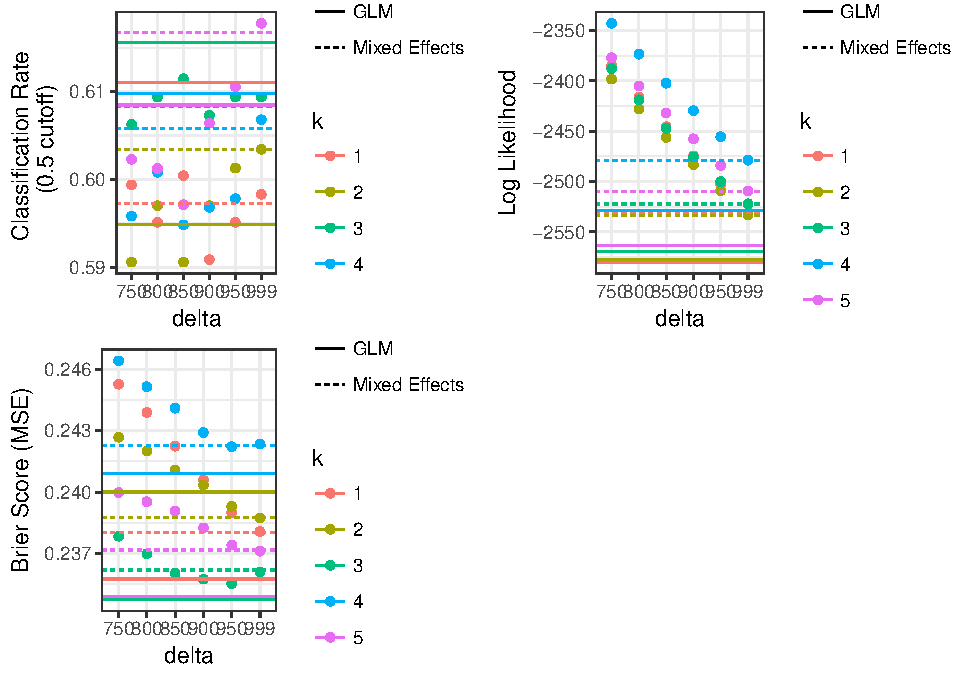
\includegraphics{thesis_files/figure-latex/home-1.pdf}

\section{One Season Only}\label{one-season-only}

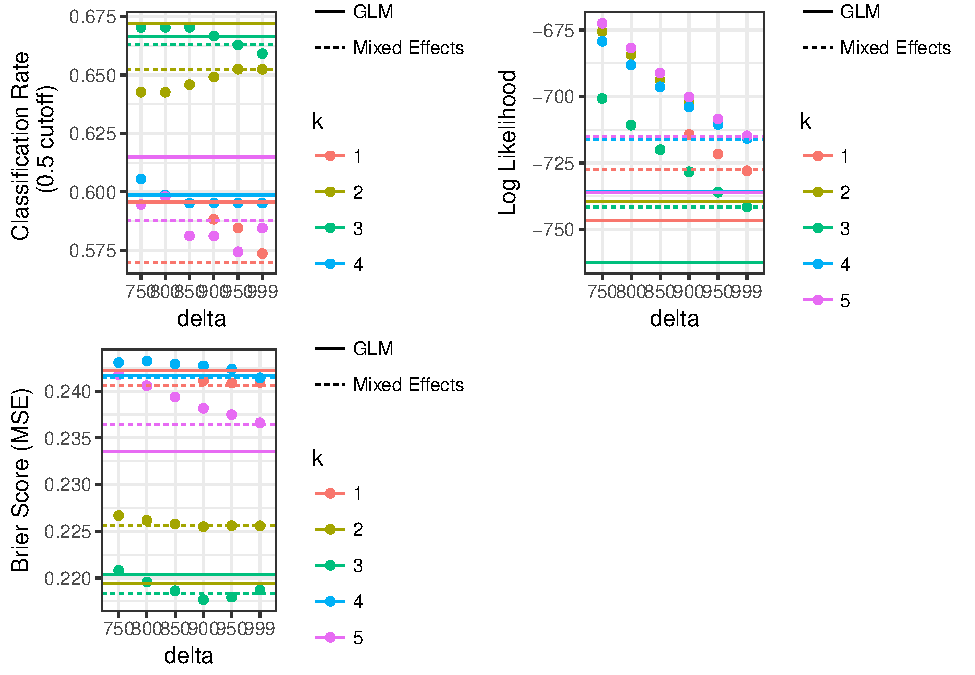
\includegraphics{thesis_files/figure-latex/2015-1.pdf}

\backmatter

\chapter*{References}\label{references}
\addcontentsline{toc}{chapter}{References}

\markboth{References}{References}

\noindent

\setlength{\parindent}{-0.20in} \setlength{\leftskip}{0.20in}
\setlength{\parskip}{8pt}

\hypertarget{refs}{}
\hypertarget{ref-albert93}{}
Albert, J. (1993). Statistical analysis of hitting streaks in baseball:
Comment. \emph{Journal of the American Statistical Association},
\emph{88}(424), 1184--1188.

\hypertarget{ref-albert13}{}
Albert, J. (2013). Looking at spacings to assess streakiness.
\emph{Journal of Quantitative Analysis in Sports}, \emph{9}(2), 1--13.

\hypertarget{ref-albert99}{}
Albert, J., \& Williamson, P. (1999). Using model/data simulations to
detect streakiness. \emph{The American Statistician}, \emph{55}, 41--50.

\hypertarget{ref-ameen84}{}
Ameen, J. R., \& Harrison, P. J. (1984). Discount weighted estimation.
\emph{Journal of Forecasting}, \emph{3}, 285--296.

\hypertarget{ref-bareli06}{}
Bar-Eli, M., Avugos, S., \& Raab, M. (2006). Twenty years of ``hot
hand'' research: Review and critique. \emph{Psychology of Sport and
Exercise}, \emph{7}, 525--553.

\hypertarget{ref-gilovich85}{}
Gilovich, T., Vallone, R., \& Tversky, A. (1985). The hot hand in
basketball: On the misperception of random sequences. \emph{Cognitive
Psychology}, \emph{17}, 295--314.

\hypertarget{ref-joseph}{}
Joseph, L. (n.d.). Specifying a new sampling distribution. Retrieved
from
\url{http://www.medicine.mcgill.ca/epidemiology/Joseph/courses/common/Tricks.html}

\hypertarget{ref-west10}{}
Prado, R., \& West, M. (2010). \emph{Time series: Modelling, Computation
\& Inference}. Chapman \& Hall/CRC Press.

\hypertarget{ref-wetzels16}{}
Wetzels, R., Tutschkow, D., Dolan, C., Sluis, S. van der, Dutilh, G., \&
Wagenmakers, E.-J. (2016). A Bayesian test for the hot hand phenomenon.
\emph{Journal of Mathematical Psychology}, \emph{72}, 200--209.


% Index?

\end{document}
